%%%%%%%%%%%%%%%%%%%%%%%%%%%%%%%%%%%%%%%%%
% The Legrand Orange Book
% LaTeX Template
% Version 2.1.1 (14/2/16)
%
% This template has been downloaded from:
% http://www.LaTeXTemplates.com
%
% Original author:
% Mathias Legrand (legrand.mathias@gmail.com) with modifications by:
% Vel (vel@latextemplates.com)
%
% License:
% CC BY-NC-SA 3.0 (http://creativecommons.org/licenses/by-nc-sa/3.0/)
%
% Compiling this template:
% This template uses biber for its bibliography and makeindex for its index.
% When you first open the template, compile it from the command line with the 
% commands below to make sure your LaTeX distribution is configured correctly:
%
% 1) pdflatex main
% 2) makeindex main.idx -s StyleInd.ist
% 3) biber main
% 4) pdflatex main x 2
%
% After this, when you wish to update the bibliography/index use the appropriate
% command above and make sure to compile with pdflatex several times 
% afterwards to propagate your changes to the document.
%
% This template also uses a number of packages which may need to be
% updated to the newest versions for the template to compile. It is strongly
% recommended you update your LaTeX distribution if you have any
% compilation errors.
%
% Important note:
% Chapter heading images should have a 2:1 width:height ratio,
% e.g. 920px width and 460px height.
%
%%%%%%%%%%%%%%%%%%%%%%%%%%%%%%%%%%%%%%%%%

%----------------------------------------------------------------------------------------
%	PACKAGES AND OTHER DOCUMENT CONFIGURATIONS
%----------------------------------------------------------------------------------------

\documentclass[10pt,fleqn,openany]{book} % Default font size and left-justified equations

%----------------------------------------------------------------------------------------

%%%%%%%%%%%%%%%%%%%%%%%%%%%%%%%%%%%%%%%%%
% The Legrand Orange Book
% Structural Definitions File
% Version 2.0 (9/2/15)
%
% Original author:
% Mathias Legrand (legrand.mathias@gmail.com) with modifications by:
% Vel (vel@latextemplates.com)
% 
% This file has been downloaded from:
% http://www.LaTeXTemplates.com
%
% License:
% CC BY-NC-SA 3.0 (http://creativecommons.org/licenses/by-nc-sa/3.0/)
%
%%%%%%%%%%%%%%%%%%%%%%%%%%%%%%%%%%%%%%%%%

%----------------------------------------------------------------------------------------
%	VARIOUS REQUIRED PACKAGES AND CONFIGURATIONS
%----------------------------------------------------------------------------------------

\usepackage[top=1cm,bottom=1cm,left=1cm,right=1cm,headsep=5pt,a5paper]{geometry} % Page margins

\usepackage{graphicx} % Required for including pictures
\graphicspath{{images/}} % Specifies the directory where pictures are stored

\usepackage{tikz} % Required for drawing custom shapes

\usepackage[english]{babel} % English language/hyphenation

\usepackage{enumitem} % Customize lists
\setlist{nolistsep} % Reduce spacing between bullet points and numbered lists

\usepackage{booktabs} % Required for nicer horizontal rules in tables

\usepackage{xcolor} % Required for specifying colors by name

\usepackage{multicol} % Required for multilines

\usepackage{pdflscape} % Required for landscape pages

\usepackage{wrapfig} % Required for wrapping text around figures

\definecolor{ocre}{RGB}{90,137,208} % Define the orange color used for highlighting throughout the book

%----------------------------------------------------------------------------------------
%	FONTS
%----------------------------------------------------------------------------------------

\usepackage{avant} % Use the Avantgarde font for headings
%\usepackage{times} % Use the Times font for headings
\usepackage{mathptmx} % Use the Adobe Times Roman as the default text font together with math symbols from the Sym­bol, Chancery and Com­puter Modern fonts

\usepackage{microtype} % Slightly tweak font spacing for aesthetics
\usepackage[utf8]{inputenc} % Required for including letters with accents
\usepackage[T1]{fontenc} % Use 8-bit encoding that has 256 glyphs

%----------------------------------------------------------------------------------------
%	BIBLIOGRAPHY AND INDEX
%----------------------------------------------------------------------------------------

\usepackage[style=alphabetic,citestyle=numeric,sorting=nyt,sortcites=true,autopunct=true,babel=hyphen,hyperref=true,abbreviate=false,backref=true,backend=biber]{biblatex}
\addbibresource{bibliography.bib} % BibTeX bibliography file
\defbibheading{bibempty}{}

\usepackage{calc} % For simpler calculation - used for spacing the index letter headings correctly
\usepackage{makeidx} % Required to make an index
\makeindex % Tells LaTeX to create the files required for indexing

%----------------------------------------------------------------------------------------
%	MAIN TABLE OF CONTENTS
%----------------------------------------------------------------------------------------

\usepackage{titletoc} % Required for manipulating the table of contents

\contentsmargin{0cm} % Removes the default margin

% Part text styling
\titlecontents{part}[0cm]
{\addvspace{20pt}\centering\large\bfseries}
{}
{}
{}

% Chapter text styling
\titlecontents{chapter}[1.25cm] % Indentation
{\addvspace{12pt}\large\sffamily\bfseries} % Spacing and font options for chapters
{\contentslabel[\Large\thecontentslabel]{1.25cm}} % Chapter number
{\color{black}}
{\color{black}\normalsize\;\titlerule*[.5pc]{.}\;\thecontentspage} % Page number

% Section text styling
\titlecontents{section}[1.25cm] % Indentation
{\addvspace{3pt}\sffamily\bfseries} % Spacing and font options for sections
{\contentslabel[\thecontentslabel]{1.25cm}} % Section number
{}
{\hfill\color{black}\thecontentspage} % Page number
[]

% Subsection text styling
\titlecontents{subsection}[1.25cm] % Indentation
{\addvspace{1pt}\sffamily\small} % Spacing and font options for subsections
{\contentslabel[\thecontentslabel]{1.25cm}} % Subsection number
{}
{\ \titlerule*[.5pc]{.}\;\thecontentspage} % Page number
[]

% List of figures
\titlecontents{figure}[0em]
{\addvspace{-5pt}\sffamily}
{\thecontentslabel\hspace*{1em}}
{}
{\ \titlerule*[.5pc]{.}\;\thecontentspage}
[]

% List of tables
\titlecontents{table}[0em]
{\addvspace{-5pt}\sffamily}
{\thecontentslabel\hspace*{1em}}
{}
{\ \titlerule*[.5pc]{.}\;\thecontentspage}
[]

%----------------------------------------------------------------------------------------
%	MINI TABLE OF CONTENTS IN PART HEADS
%----------------------------------------------------------------------------------------

% Chapter text styling
\titlecontents{lchapter}[0em] % Indenting
{\addvspace{15pt}\large\sffamily\bfseries} % Spacing and font options for chapters
{\color{ocre}\contentslabel[\Large\thecontentslabel]{1.25cm}\color{ocre}} % Chapter number
{}  
{\color{ocre}\normalsize\sffamily\bfseries\;\titlerule*[.5pc]{.}\;\thecontentspage} % Page number

% Section text styling
\titlecontents{lsection}[0em] % Indenting
{\sffamily\small} % Spacing and font options for sections
{\contentslabel[\thecontentslabel]{1.25cm}} % Section number
{}
{}

% Subsection text styling
\titlecontents{lsubsection}[.5em] % Indentation
{\normalfont\footnotesize\sffamily} % Font settings
{}
{}
{}

%----------------------------------------------------------------------------------------
%	THEOREM STYLES
%----------------------------------------------------------------------------------------

\usepackage{amsmath,amsfonts,amssymb,amsthm} % For math equations, theorems, symbols, etc

\newcommand{\intoo}[2]{\mathopen{]}#1\,;#2\mathclose{[}}
\newcommand{\ud}{\mathop{\mathrm{{}d}}\mathopen{}}
\newcommand{\intff}[2]{\mathopen{[}#1\,;#2\mathclose{]}}
\newtheorem{notation}{Notation}[chapter]

% Boxed/framed environments
\newtheoremstyle{ocrenumbox}% % Theorem style name
{0pt}% Space above
{0pt}% Space below
{\normalfont}% % Body font
{}% Indent amount
{\small\bf\sffamily\color{ocre}}% % Theorem head font
{\;}% Punctuation after theorem head
{0.25em}% Space after theorem head
{\small\sffamily\color{ocre}\thmname{#1}\nobreakspace\thmnumber{\@ifnotempty{#1}{}\@upn{#2}}% Theorem text (e.g. Theorem 2.1)
\thmnote{\nobreakspace\the\thm@notefont\sffamily\bfseries\color{black}---\nobreakspace#3.}} % Optional theorem note
\renewcommand{\qedsymbol}{$\blacksquare$}% Optional qed square

\newtheoremstyle{blacknumex}% Theorem style name
{5pt}% Space above
{5pt}% Space below
{\normalfont}% Body font
{} % Indent amount
{\small\bf\sffamily}% Theorem head font
{\;}% Punctuation after theorem head
{0.25em}% Space after theorem head
{\small\sffamily{\tiny\ensuremath{\blacksquare}}\nobreakspace\thmname{#1}\nobreakspace\thmnumber{\@ifnotempty{#1}{}\@upn{#2}}% Theorem text (e.g. Theorem 2.1)
\thmnote{\nobreakspace\the\thm@notefont\sffamily\bfseries---\nobreakspace#3.}}% Optional theorem note

\newtheoremstyle{blacknumbox} % Theorem style name
{0pt}% Space above
{0pt}% Space below
{\normalfont}% Body font
{}% Indent amount
{\small\bf\sffamily}% Theorem head font
{\;}% Punctuation after theorem head
{0.25em}% Space after theorem head
{\small\sffamily\thmname{#1}\nobreakspace\thmnumber{\@ifnotempty{#1}{}\@upn{#2}}% Theorem text (e.g. Theorem 2.1)
\thmnote{\nobreakspace\the\thm@notefont\sffamily\bfseries---\nobreakspace#3.}}% Optional theorem note

% Non-boxed/non-framed environments
\newtheoremstyle{ocrenum}% % Theorem style name
{5pt}% Space above
{5pt}% Space below
{\normalfont}% % Body font
{}% Indent amount
{\small\bf\sffamily\color{ocre}}% % Theorem head font
{\;}% Punctuation after theorem head
{0.25em}% Space after theorem head
{\small\sffamily\color{ocre}\thmname{#1}\nobreakspace\thmnumber{\@ifnotempty{#1}{}\@upn{#2}}% Theorem text (e.g. Theorem 2.1)
\thmnote{\nobreakspace\the\thm@notefont\sffamily\bfseries\color{black}---\nobreakspace#3.}} % Optional theorem note
\renewcommand{\qedsymbol}{$\blacksquare$}% Optional qed square
\makeatother

% Defines the theorem text style for each type of theorem to one of the three styles above
\newcounter{dummy} 
\numberwithin{dummy}{section}
\theoremstyle{ocrenumbox}
\newtheorem{theoremeT}[dummy]{Theorem}
\newtheorem{problem}{Problem}[chapter]
\newtheorem{exerciseT}{Exercise}[chapter]
\theoremstyle{blacknumex}
\newtheorem{exampleT}{Example}[chapter]
\theoremstyle{blacknumbox}
\newtheorem{vocabulary}{Vocabulary}[chapter]
\newtheorem{definitionT}{Definition}[section]
\newtheorem{corollaryT}[dummy]{Corollary}
\theoremstyle{ocrenum}
\newtheorem{proposition}[dummy]{Proposition}

%----------------------------------------------------------------------------------------
%	DEFINITION OF COLORED BOXES
%----------------------------------------------------------------------------------------

\RequirePackage[framemethod=default]{mdframed} % Required for creating the theorem, definition, exercise and corollary boxes

% Theorem box
\newmdenv[skipabove=7pt,
skipbelow=7pt,
backgroundcolor=black!5,
linecolor=ocre,
innerleftmargin=5pt,
innerrightmargin=5pt,
innertopmargin=5pt,
leftmargin=0cm,
rightmargin=0cm,
innerbottommargin=5pt]{tBox}

% Exercise box	  
\newmdenv[skipabove=7pt,
skipbelow=7pt,
rightline=false,
leftline=true,
topline=false,
bottomline=false,
backgroundcolor=ocre!10,
linecolor=ocre,
innerleftmargin=5pt,
innerrightmargin=5pt,
innertopmargin=5pt,
innerbottommargin=5pt,
leftmargin=0cm,
rightmargin=0cm,
linewidth=4pt]{eBox}	

% Definition box
\newmdenv[skipabove=7pt,
skipbelow=7pt,
rightline=false,
leftline=true,
topline=false,
bottomline=false,
linecolor=ocre,
innerleftmargin=5pt,
innerrightmargin=5pt,
innertopmargin=0pt,
leftmargin=0cm,
rightmargin=0cm,
linewidth=4pt,
innerbottommargin=0pt]{dBox}	

% Corollary box
\newmdenv[skipabove=7pt,
skipbelow=7pt,
rightline=false,
leftline=true,
topline=false,
bottomline=false,
linecolor=gray,
backgroundcolor=black!5,
innerleftmargin=5pt,
innerrightmargin=5pt,
innertopmargin=5pt,
leftmargin=0cm,
rightmargin=0cm,
linewidth=4pt,
innerbottommargin=5pt]{cBox}

% Creates an environment for each type of theorem and assigns it a theorem text style from the "Theorem Styles" section above and a colored box from above
\newenvironment{theorem}{\begin{tBox}\begin{theoremeT}}{\end{theoremeT}\end{tBox}}
\newenvironment{exercise}{\begin{eBox}\begin{exerciseT}}{\hfill{\color{ocre}\tiny\ensuremath{\blacksquare}}\end{exerciseT}\end{eBox}}				  
\newenvironment{definition}{\begin{dBox}\begin{definitionT}}{\end{definitionT}\end{dBox}}	
\newenvironment{example}{\begin{exampleT}}{\hfill{\tiny\ensuremath{\blacksquare}}\end{exampleT}}		
\newenvironment{corollary}{\begin{cBox}\begin{corollaryT}}{\end{corollaryT}\end{cBox}}	

%----------------------------------------------------------------------------------------
%	REMARK ENVIRONMENT
%----------------------------------------------------------------------------------------

\newenvironment{remark}{\par\vspace{10pt}\small % Vertical white space above the remark and smaller font size
\begin{list}{}{
\leftmargin=35pt % Indentation on the left
\rightmargin=25pt}\item\ignorespaces % Indentation on the right
\makebox[-2.5pt]{\begin{tikzpicture}[overlay]
\node[draw=ocre!60,line width=1pt,circle,fill=ocre!25,font=\sffamily\bfseries,inner sep=2pt,outer sep=0pt] at (-15pt,0pt){\textcolor{ocre}{R}};\end{tikzpicture}} % Orange R in a circle
\advance\baselineskip -1pt}{\end{list}\vskip5pt} % Tighter line spacing and white space after remark

%----------------------------------------------------------------------------------------
%	SECTION NUMBERING IN THE MARGIN
%----------------------------------------------------------------------------------------

\makeatletter
\renewcommand{\@seccntformat}[1]{\llap{\textcolor{black}{}\hspace{1em}}}      
\renewcommand{\section}{\@startsection{section}{1}{\z@}
{-4ex \@plus -1ex \@minus -.4ex}
{1ex \@plus.2ex }
{\normalfont\large\sffamily\bfseries}}
\renewcommand{\subsection}{\@startsection {subsection}{2}{\z@}
{-3ex \@plus -0.1ex \@minus -.4ex}
{0.5ex \@plus.2ex }
{\normalfont\sffamily\bfseries}}
\renewcommand{\subsubsection}{\@startsection {subsubsection}{3}{\z@}
{-2ex \@plus -0.1ex \@minus -.2ex}
{.2ex \@plus.2ex }
{\normalfont\small\sffamily\bfseries}}                        
\renewcommand\paragraph{\@startsection{paragraph}{4}{\z@}
{-2ex \@plus-.2ex \@minus .2ex}
{.1ex}
{\normalfont\small\sffamily\bfseries}}

%----------------------------------------------------------------------------------------
%	PART HEADINGS
%----------------------------------------------------------------------------------------

% numbered part in the table of contents
\newcommand{\@mypartnumtocformat}[2]{%
\setlength\fboxsep{0pt}%
\noindent\colorbox{ocre!20}{\strut\parbox[c][.7cm]{\ecart}{\color{ocre!70}\Large\sffamily\bfseries\centering#1}}\hskip\esp\colorbox{ocre!40}{\strut\parbox[c][.7cm]{\linewidth-\ecart-\esp}{\Large\sffamily\centering#2}}}%
%%%%%%%%%%%%%%%%%%%%%%%%%%%%%%%%%%
% unnumbered part in the table of contents
\newcommand{\@myparttocformat}[1]{%
\setlength\fboxsep{0pt}%
\noindent\colorbox{ocre!40}{\strut\parbox[c][.7cm]{\linewidth}{\Large\sffamily\centering#1}}}%
%%%%%%%%%%%%%%%%%%%%%%%%%%%%%%%%%%
\newlength\esp
\setlength\esp{4pt}
\newlength\ecart
\setlength\ecart{1.2cm-\esp}
\newcommand{\thepartimage}{}%
\newcommand{\partimage}[1]{\renewcommand{\thepartimage}{#1}}%
\def\@part[#1]#2{%
\ifnum \c@secnumdepth >-2\relax%
\refstepcounter{part}%
\addcontentsline{toc}{part}{\texorpdfstring{\protect\@mypartnumtocformat{\thepart}{#1}}{\partname~\thepart\ ---\ #1}}
\else%
\addcontentsline{toc}{part}{\texorpdfstring{\protect\@myparttocformat{#1}}{#1}}%
\fi%
\startcontents%
\markboth{}{}%
{
\begin{tikzpicture}[remember picture,overlay]%
\node at (current page.north west){\begin{tikzpicture}[remember picture,overlay]%	
\fill[ocre!20](0cm,0cm) rectangle (\paperwidth,-\paperheight);
\node[anchor=north] at (4cm,-3.25cm){\color{ocre!40}\fontsize{220}{100}\sffamily\bfseries\@Roman\c@part}; 
\node[anchor=south east] at (\paperwidth-1cm,-\paperheight+1cm){\parbox[t][][t]{8.5cm}{
\printcontents{l}{0}{\setcounter{tocdepth}{1}}%
}};
\node[anchor=north east] at (\paperwidth-1.5cm,-3.25cm){\parbox[t][][t]{15cm}{\strut\raggedleft\color{white}\fontsize{30}{30}\sffamily\bfseries#2}};
\end{tikzpicture}};
\end{tikzpicture}}%
\@endpart}
\def\@spart#1{%
\startcontents%
\phantomsection
{
\begin{tikzpicture}[remember picture,overlay]%
\node at (current page.north west){\begin{tikzpicture}[remember picture,overlay]%	
\fill[ocre!20](0cm,0cm) rectangle (\paperwidth,-\paperheight);
\node[anchor=north east] at (\paperwidth-1.5cm,-3.25cm){\parbox[t][][t]{15cm}{\strut\raggedleft\color{white}\fontsize{30}{30}\sffamily\bfseries#1}};
\end{tikzpicture}};
\end{tikzpicture}}
\addcontentsline{toc}{part}{\texorpdfstring{%
\setlength\fboxsep{0pt}%
\noindent\protect\colorbox{ocre!40}{\strut\protect\parbox[c][.7cm]{\linewidth}{\Large\sffamily\protect\centering #1\quad\mbox{}}}}{#1}}%
\@endpart}
\def\@endpart{\vfil\newpage
\if@twoside
\if@openright
\null
\newpage
\fi
\fi
\if@tempswa
\twocolumn
\fi}

%----------------------------------------------------------------------------------------
%	CHAPTER HEADINGS
%----------------------------------------------------------------------------------------

% A switch to conditionally include a picture, implemented by  Christian Hupfer
\newif\ifusechapterimage
\usechapterimagetrue
\newcommand{\thechapterimage}{}%
\newcommand{\chapterimage}[1]{\ifusechapterimage\renewcommand{\thechapterimage}{#1}\fi}%
\def\@makechapterhead#1{%
{\parindent \z@ \raggedright \normalfont
\ifnum \c@secnumdepth >\m@ne
\if@mainmatter
\begin{tikzpicture}[remember picture,overlay]
\node at (current page.north west)
{\begin{tikzpicture}[remember picture,overlay]
\node[anchor=north west,inner sep=0pt] at (0,0) {\ifusechapterimage\includegraphics[width=\paperwidth]{\thechapterimage}\fi};
\draw[anchor=west] (\Gm@lmargin,-5cm) node [line width=2pt,rounded corners=15pt,draw=ocre,fill=white,fill opacity=0.5,inner sep=15pt]{\strut\makebox[22cm]{}};
\draw[anchor=west] (\Gm@lmargin+.3cm,-5cm) node {\huge\sffamily\bfseries\color{black}#1\strut};
\end{tikzpicture}};
\end{tikzpicture}
\else
\begin{tikzpicture}[remember picture,overlay]
\node at (current page.north west)
{\begin{tikzpicture}[remember picture,overlay]
\node[anchor=north west,inner sep=0pt] at (0,0) {\ifusechapterimage\includegraphics[width=\paperwidth]{\thechapterimage}\fi};
\draw[anchor=west] (\Gm@lmargin,-5cm) node [line width=2pt,rounded corners=15pt,draw=ocre,fill=white,fill opacity=0.5,inner sep=15pt]{\strut\makebox[22cm]{}};
\draw[anchor=west] (\Gm@lmargin+.3cm,-5cm) node {\huge\sffamily\bfseries\color{black}#1\strut};
\end{tikzpicture}};
\end{tikzpicture}
\fi\fi\par\vspace*{130\p@}}}

%-------------------------------------------

\def\@makeschapterhead#1{%
\begin{tikzpicture}[remember picture,overlay]
\node at (current page.north west)
{\begin{tikzpicture}[remember picture,overlay]
\node[anchor=north west,inner sep=0pt] at (0,0) {\ifusechapterimage\includegraphics[width=\paperwidth]{\thechapterimage}\fi};
\draw[anchor=west] (\Gm@lmargin,-5cm) node [line width=2pt,rounded corners=15pt,draw=ocre,fill=white,fill opacity=0.5,inner sep=15pt]{\strut\makebox[22cm]{}};
\draw[anchor=west] (\Gm@lmargin+.3cm,-5cm) node {\huge\sffamily\bfseries\color{black}#1\strut};
\end{tikzpicture}};
\end{tikzpicture}
\par\vspace*{130\p@}}
\makeatother

%----------------------------------------------------------------------------------------
%	FANCY AND PAGE NUMERATION
%----------------------------------------------------------------------------------------

\usepackage{fancyhdr}
\lfoot{}
\cfoot{}
\rfoot{}
\lhead[\thepage]{{
\includegraphics[width=0.3cm]{icon_bicolor}}}
\chead{\textbf{\leftmark}}
\rhead[{
\includegraphics[width=0.3cm]{icon_bicolor}}]{\thepage}
\renewcommand{\headrulewidth}{0.5pt}
\renewcommand{\footrulewidth}{0pt}
\renewcommand{\chaptermark}[1]{\markboth{#1}{}}

\setlength\headsep{10pt}

\fancypagestyle{plain}
{
	\fancyhf{}
	\lhead{}
	\chead{}
	\rhead{}
	\lfoot{}
	\cfoot{}
	\rfoot{}
}

%----------------------------------------------------------------------------------------
%	HYPERLINKS IN THE DOCUMENTS
%----------------------------------------------------------------------------------------

\usepackage{hyperref}
\hypersetup{hidelinks,backref=true,pagebackref=true,hyperindex=true,colorlinks=false,breaklinks=true,urlcolor= ocre,bookmarks=true,bookmarksopen=false,pdftitle={Title},pdfauthor={Author}}
\usepackage{bookmark}
\bookmarksetup{
open,
numbered,
addtohook={%
\ifnum\bookmarkget{level}=0 % chapter
\bookmarksetup{bold}%
\fi
\ifnum\bookmarkget{level}=-1 % part
\bookmarksetup{color=ocre,bold}%
\fi
}
}

%----------------------------------------------------------------------------------------
%	CUSTOM FUNCS
%----------------------------------------------------------------------------------------

%	PAPERS ABSTRACTS
\newcommand{\paperabstract}[4]{
	\vspace*{10pt}
	\item \textbf{#1}. #2
	\\
	\textit{#3}
	\vspace*{10pt}
	\\
	#4
}

%	POSTERS
\newcommand{\poster}[3]{
	\vspace*{10pt}
	\item #1
	\\
	\textit{#2}
	\\
	\textit{#3}
}

%   INTEXT FIGURE
\usepackage{float}

\newcommand{\intextfigure}[1]{
	\begin{figure}[!htb]
		\begin{center}
			\includegraphics[width=\paperwidth - 4cm]{#1}
		\end{center}
	\end{figure}
}

\usepackage{linednotes} % Insert the commands.tex file which contains the majority of the structure behind the template

\begin{document}

%----------------------------------------------------------------------------------------
%	COVER FRONT PAGE
%----------------------------------------------------------------------------------------

\begingroup
\thispagestyle{empty}
\begin{tikzpicture}[remember picture,overlay]
\coordinate (midpoint) at (current page.north);
\node at (current page.north west)
{\begin{tikzpicture}[remember picture,overlay]
	\node[anchor=north west,inner sep=0pt] at (0,0) {
\includegraphics[width=\paperwidth]{cover_3}}; % Background image
	\end{tikzpicture}};
\end{tikzpicture}
\vfill
\endgroup


%----------------------------------------------------------------------------------------
%	COPYRIGHT PAGE
%----------------------------------------------------------------------------------------

\newpage
~\vfill
\thispagestyle{empty}

\noindent \textsc{Copyright \copyright\ 2017 National Research Nuclear University ``MEPhI''}\\

\noindent \textsc{Licensed under the Creative Commons Attribution-NoDerivatives 4.0 International license}\\

\noindent \textsc{https://creativecommons.org/licenses/by-nd/4.0}\\

\noindent \textsc{Authors: Chernyshov Artyom, Aleksandr Panov}\\

\noindent \textsc{Designer: Ilya Sukonkin }\\

\noindent \textsc{Editors: Alexei Samsonovich, Valentin Klimov}\\

\noindent \textsc{Conference site: http://bica2017.bicasociety.org//}\\

\noindent \textit{August 2017}

%----------------------------------------------------------------------------------------
%	TABLE OF CONTENTS
%----------------------------------------------------------------------------------------

%\usechapterimagefalse % If you don't want to include a chapter image, use this to toggle images off - it can be enabled later with \usechapterimagetrue

\chapterimage{00_head_content}

\pagestyle{empty} % No headers

\tableofcontents % Print the table of contents itself

\pagestyle{fancy}

%----------------------------------------------------------------------------------------
%	CHAPTER 1
%----------------------------------------------------------------------------------------

\chapterimage{01_head_welcome}

\chapter{Welcome to BICA 2017}

The challenge to replicate all the key features of the human mind in a digital environment using a biologically inspired approach (the BICA Challenge) is the spirit and the core of the new frontier that every year attracts more and more young scientists. Its counterpart challenge of Cybersecurity acquires priority as we advance deeper and deeper into the uncharted territory. After many decades of progress in the field of artificial intelligence, problems that we are facing today require a fresh, multidisciplinary view. We need to learn from scratch how to achieve goals that could never be taken seriously in the past, with an understanding that a novel approach is necessary, because essential qualities of biological intelligent systems like robustness, flexibility, adaptability, communicability, and reliability are still unmatched by their artificial counterparts.

This brochure serves as a participant guide for two events, taking place back-to-back at the same location: (1) the First International Early Research Career Enhancement School (FIERCES) on Biologically Inspired Cognitive Architectures and Cybersecurity, which is the second meeting of the FIERCES series, and (2) The 2017 Annual International Conference on Biologically Inspired Cognitive Architectures, also known as the Eighth Annual Meeting of the BICA Society. The events are being held in Baltschug Kempinski hotel in Moscow, Russia, during August 1-6, 2017. Their mission is to facilitate the interaction and collaboration among top experts in the field (including such names as Agnese Augello, Olivier Georgeon, Ricardo Gudwin, Ignazio Infantino, Frank Krueger, Adriano Manfre', Giovanni Pilato, Aaron Sloman, Filippo Vella) and young researchers, who devoted themselves to solution of the BICA Challenge, by bridging cross-disciplinary, cross-generation and cross-cultural barriers.

Biologically Inspired Cognitive Architectures (BICA) are computational blueprints for building artificial intelligent agents, inspired from natural prototypes. They help us to utilize the vast accumulated knowledge about the brain in order to learn from nature how to build intelligent systems. At the same time, new techniques and concepts complement the main focus of the forum. As a consequence, this double-event becomes highly interdisciplinary in nature and will yield bi-directional flow of understanding between experts in all involved disciplines.

Therefore, topics of talks and posters included in the program and in the accompanying electronic volume extensively cover the most advanced scientific fields relevant to BICA that are traditionally considered at the international level of significance and discussed at many mainstream national and international conferences on artificial intelligence, neuroscience and cognitive modeling, including conferences organized by BICA Society. The list of the latter is quite long. Beginning with the AAAI Fall Symposia on BICA (2008, 2009), the Annual International Conference on BICA has been held every year since 2010, demonstrating progressively growing popularity. Locations of the conference included Washington, DC (2010); Palermo, Italy (2012); Kiev, Ukraine (2013); Cambridge, Massachusets (2014); Lyon, France (2015); and New York, USA (2016). The 2017 BICA event in Moscow, however, is unique in its kind, because it brings the conference and the school together.

In this year we received a record number of qualified submissions for a BICA event, that were carefully peer-reviewed. Not all of them were included in the program. Among those, selected papers were selected for publication in prestigious venues, indexed in Web of Science and Scopus. These publication venues include a special volume of Procedia Computer Science and a special volume of Springer Series “Advances in Intelligent Systems and Computing”. In selecting those papers, we paid attention to their scientific quality and relevance to the above challenges. 

All published works have been carefully peer-reviewed and refereed, and reflect the high level of ongoing research and development in participating leading universities and research centers around the world, including those the US, in France, Germany, Italy, Spain, Japan, Brazil, China, Ukraine, Belarus, and also in Russia (Moscow, St. Petersburg, Novosibirsk and other Russian cities). The list of our Reviewers was equally widely distributed around the globe. Some good papers were recommended for publication in the journal Biologically Inspired Cognitive Architectures. We are grateful to all Authors and Reviewers for their great job.

-----

BICA / FIERCES 2017 Organizers

\section{Fierces on BICA 2017 and BICA 2017 Sponsor}
\begin{itemize}
	\item Russian Science Foundation
\end{itemize}

\section{Co-organizers}
\begin{itemize}
	\item National Research Nuclear University MEPhI
	\item BICA Society
	\item Russian Association for Artificial Intelligence
	\item Institute for Cyber Intelligence Systems
	\item Whole Brain Architecture Initiative
\end{itemize}

\section{Points of Contact}

\begin{itemize}
	\item Alexei Samsonovich
		\begin{description}
			\item[Organization] George Mason University (USA), MEPhI (Moscow)
			\item[E-mail] asamsono@gmu.edu
		\end{description} 
	\item Valentin V. Klimov
		\begin{description}
			\item[Organization] MEPhI (Moscow)
			\item[E-mail]  vvklimov@mephi.ru
		\end{description} 

\end{itemize}

%----------------------------------------------------------------------------------------
%	CHAPTER 2
%----------------------------------------------------------------------------------------

\chapterimage{02_head_program}

\chapter{Program}

Registration table opens at 8:00 AM on each day. Participants need to pre-register online in advance. Each lecture will last 45 minutes (including 15 minutes for questions and discussion) on the School and 30 minutes (including 10 minutes for questions and discussion) on the Conference. The Opening Keynotes will last one hour. Posters will be presented during all coffee breaks nad lunches. Each poster presenter will be expected to give a two-min Lightning Summary with slides during the Poster Summaries session. Canceled lectures may be replaced with ad hoc Round Tables or Special Interest Discussion Panels.

\section{Social events}
    The following social events are expected, as parts of the Conference and the School (participation is voluntary):
\begin{itemize}
    \item Anna Karenina: Ballet at Bolshoi on Monday
    \item Ostankinskaya tower: Dinner at the altitude 330M above the ground	on Tuesday
    \item Banquet-on-a-Boat: Moskva river cruise on Wednesday
    \item Welcome Reception at the Baltschug Library on Thursday
    \item Banquet at the restaurant	Ruski (85th floor) on Friday
    \item Nikulin Circus on Saturday
    \item Kremlin, Moscow bus tour and art museums on Sunday
\end{itemize}
\vfill

\section{Program-At-A-Glance}
	\vspace{10pt}
	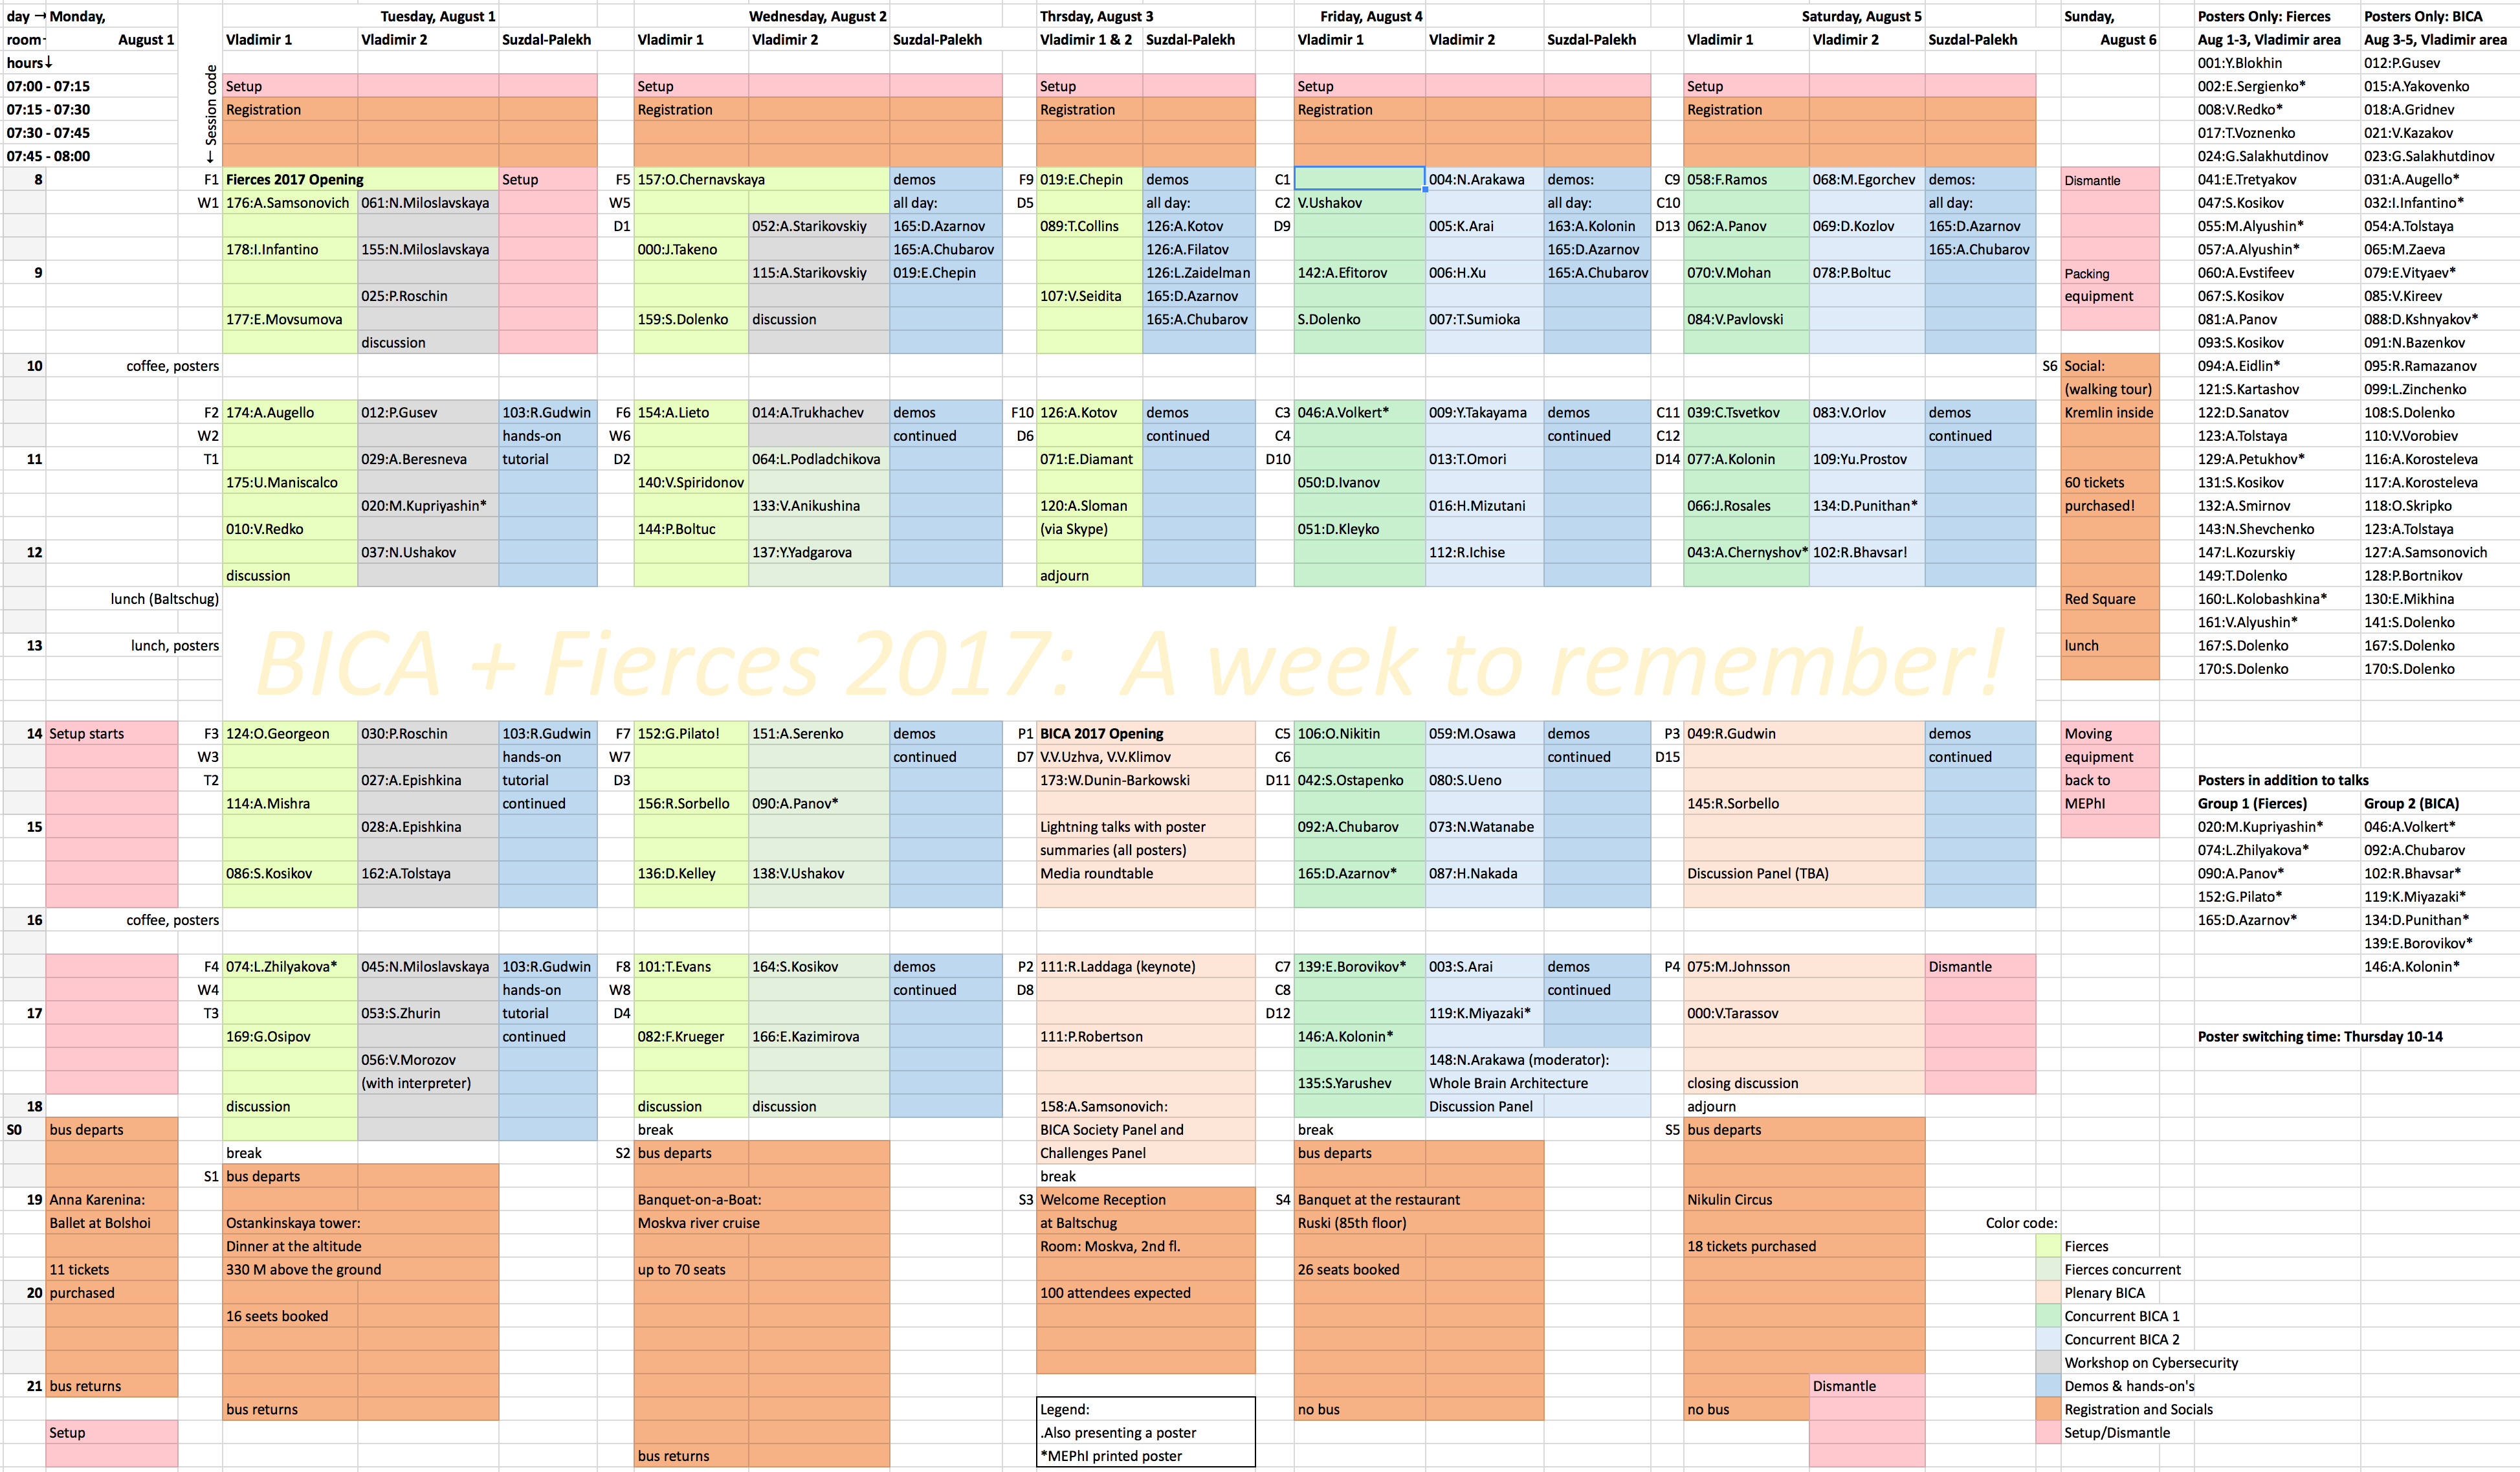
\includegraphics[angle=90,origin=c,width=0.85\textwidth]{02_detail_program}
	\vfill
	

\section{Detailed Fierces on BICA 2017 Program}
	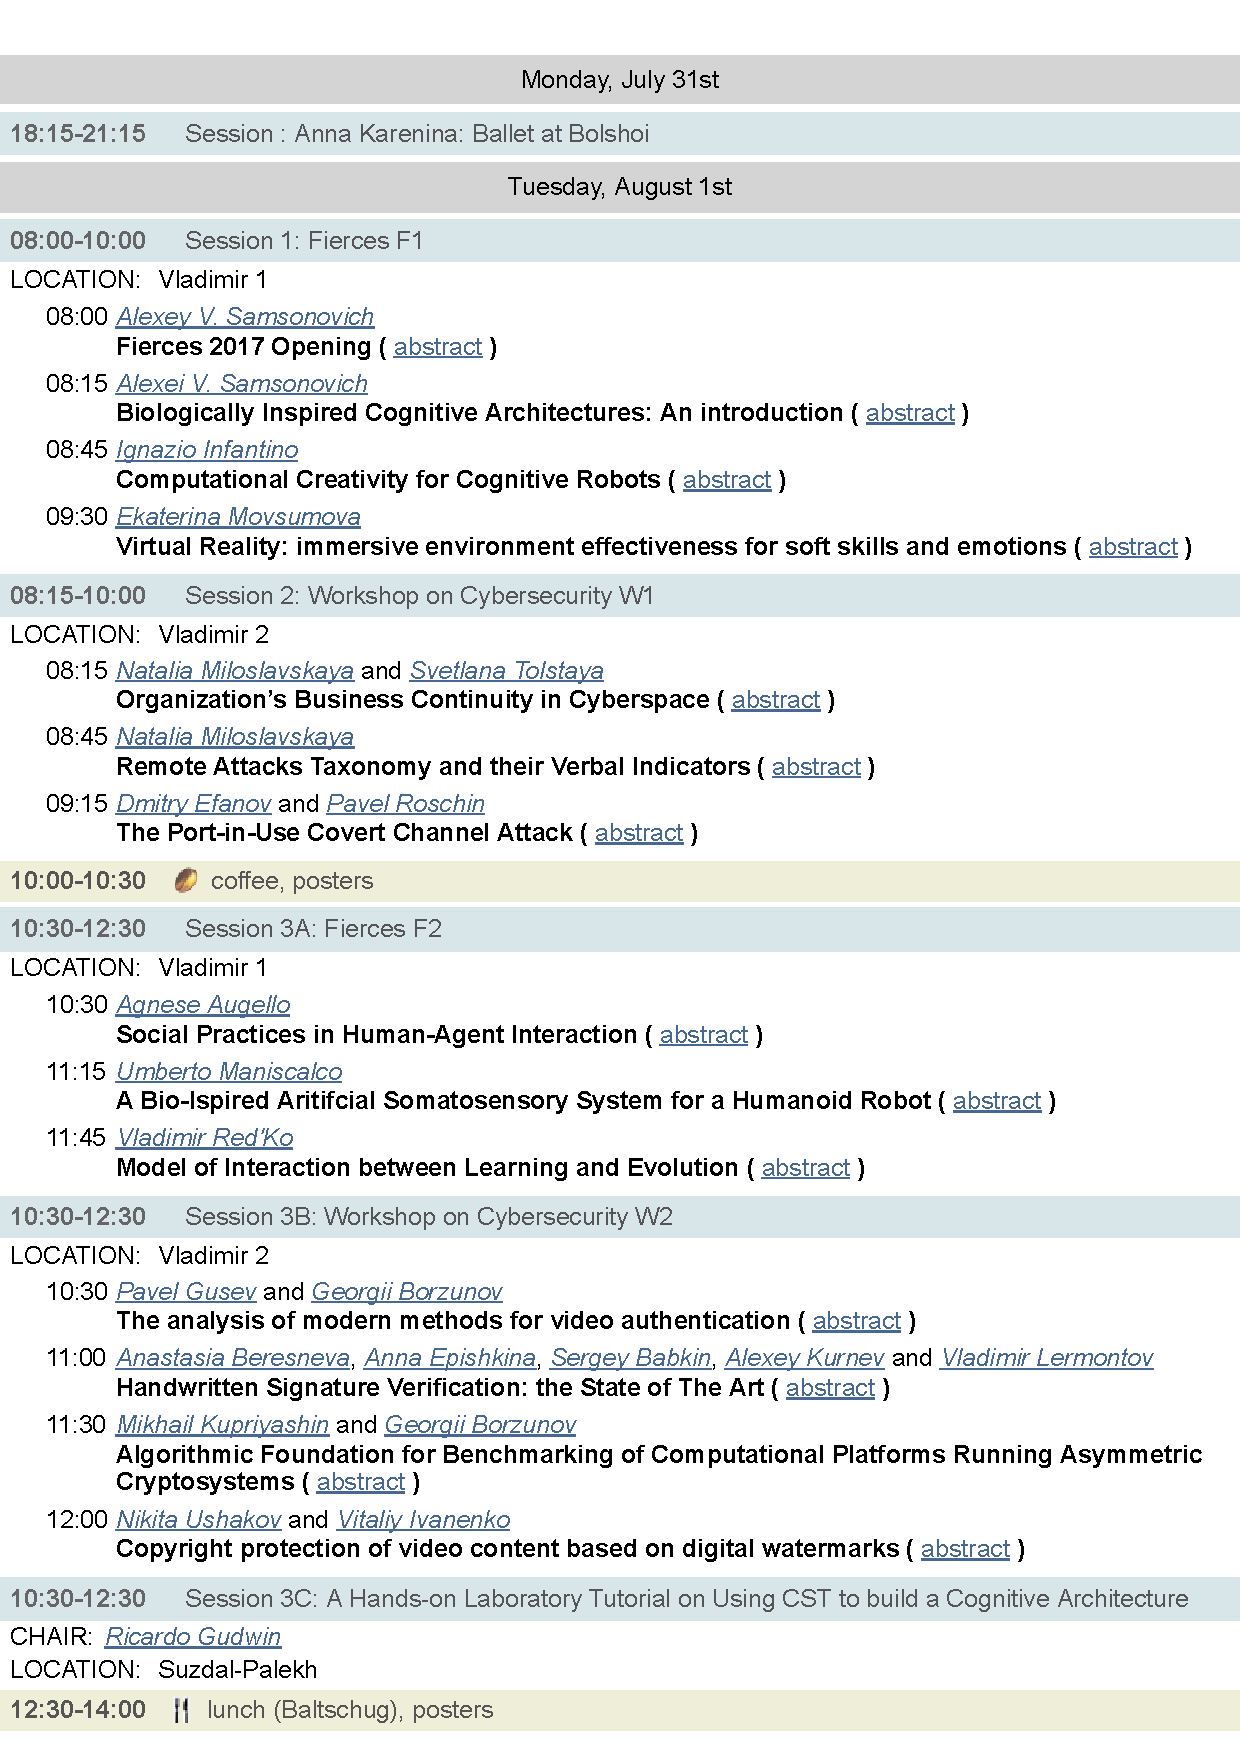
\includegraphics[width=\textwidth, page=1]{02_full_program}
	\vfill
	\includegraphics[width=\textwidth, page=2]{02_full_program}
	\vfill
	\includegraphics[width=\textwidth, page=3]{02_full_program}
	\vfill
	\includegraphics[width=\textwidth, page=4]{02_full_program}
	\vfill
	\includegraphics[width=\textwidth, page=5]{02_full_program}
	\vfill
\section{Detailed BICA 2017 Program}	

	\includegraphics[width=\textwidth, page=6]{02_full_program}
	\vfill
	\includegraphics[width=\textwidth, page=7]{02_full_program}
	\vfill
	\includegraphics[width=\textwidth, page=8]{02_full_program}
	\vfill
	\includegraphics[width=\textwidth, page=9]{02_full_program}
	\vfill
%----------------------------------------------------------------------------------------
%	CHAPTER 3
%----------------------------------------------------------------------------------------

\chapterimage{03_head_venue}

\chapter{Venue}

The Conference and the School venue is the Hotel Baltschug Kempinski, Moscow, Russia. The five-star Hotel offers spectacular views of the Kremlin and St Basil’s Cathedral. The property is located across from the Moskva River, and is nearby Moscow’s fascinating sights and premier attractions.

\intextfigure{03_hotel_around}

\intextfigure{03_hotel_inside}


The building dates back to 1898, and features contemporary décor and up-to-the-minute amenities. The hotel has 227 elegant rooms, including 36 suites and unique Design Suites. Hotel Baltschug Kempinski Moscow boasts restaurant The Baltschug Grill, as well as the refined Café Kranzler, Lobby Lounge bar, Beauty Centre Baltschug and a Health Club. In addition, there are 12 modern meeting rooms, and most offer great views over the Red Square. 

\par\bigskip
\par\bigskip
\par\bigskip
\par\bigskip
\par\bigskip
\intextfigure{03_hotel_13f}

\begin{description}
	\item[Phone] +7 495 287 2000
	\item[Email] info.baltschug@kempinski.com
	\item[Web] https://www.kempinski.com/en/moscow/hotel-baltschug
	\item[Address] Ul. Balchug 1, 115035, Moscow, Russian
\end{description}



%----------------------------------------------------------------------------------------
%	CHAPTER 4
%----------------------------------------------------------------------------------------

\chapterimage{04_head_moving_around}

\chapter{Moving around}

\section{Recommended museums, art galleries, and parks}

\begin{enumerate}
	\item The State Historical Museum
		\begin{description}
			\item[Web-site] www.shm.ru/en/
			\item[Address] 1, Red Square, Moscow, 103012, Russia 
			\item[Transport] Metro Stations Okhotny Ryad, Ploshad Revolutsii, Teatralnaya Ploshad
			\item[Opening hours] Daily from 11.00 to 19.00, closed on Tuesdays
		\end{description}

	\item 	Yuri Orlov Palaeontological Museum
		\begin{description}
			\item[Web-site] http://www.paleo.ru/museum/ 
			\item[Address] 123, Profsoyuznaya Ulitsa, Moscow, 117647, Russia 
			\item[Transport] From Teply Stan Metro station it's one stop on any form of transport, or 5-7 minutes on foot.
			\item[Opening hours] Wednesday to Friday - 10:00 to 16:00, Saturday and Sunday - 10:00 to 18:45, closed Monday and Tuesday
		\end{description}

	\item Moscow State University Zoological Museum
		\begin{description}
			\item[Web-site] http://zmmu.msu.ru/en
			\item[Address] 6, Bol'shaya Nikitskaya ulitsa, Moscow, 103009, Russia 
			\item[Transport] Okhotny Ryad or Aleksandrovsky Sad Metro stations
			\item[Opening hours] Tuesday to Sunday - 10:00 to 17:00. Monday - closed. The museum is closed on the last Tuesday of each month
		\end{description}

	\item Cosmonautics Memorial Museum
		\begin{description}
			\item[Web-site] http://www.kosmo-museum.ru/
			\item[Address] 111, Prospekt Mira, Moscow, 129515, Russia 
			\item[Transport] VDNKh Metro station
			\item[Opening hours] Daily - 10:00 to 18:00, except Mondays and the last Friday of each month
		\end{description}
	
	\item Andrei Rublev Museum of Ancient Russian Art
			\begin{description}
				\item[Web-site] http://www.rublev-museum.ru/ 
				\item[Address] 10, Andronevskaya Ploshad, Moscow, 105120, Russia 
				\item[Transport] Ploshad' Il'icha and Taganskaya Metro stations
				\item[Opening hours] 11:00 to 18:00, except Wednesdays and the last Friday of each month
			\end{description}
			
	\item State Tretyakov Gallery
	\begin{description}
		\item[Web-site] http://www.tretyakovgallery.com
		\begin{itemize}
			\item Main Gallery
				\begin{description}
					\item[Address] 10, Lavrunshkensky Pereulok, Moscow, 119017, Russia 
					\item[Transport] Tretyakovskaya or Novokuznetskaya Metro stations
			    \end{description}
   			\item House of Artists
	   			\begin{description}
					\item[Address] 10/4, Ulitsa Krymsky Val, Moscow, 119049, Russia 
					\item[Transport] From Park Kulturi or Oktyabr'skaya Metro station take trolleybuses 10 or B to the Central Park of Culture and Leisure stop
	   			\end{description}
		\end{itemize}
		\item[Opening hours] Daily from 10:00 – 19:00 (20:00), except Mondays 
	\end{description}
	
	\item State Pushkin Museum of Visual Art
		\begin{description}
			\item[Web-site] http://www.arts-museum.ru/
			\item[Address] 12, Ulitsa Volkhonka, Moscow, 121019, Russia 
			\item[Transport] Kropotkinskaya Metro station
			\item[Opening hours] Tuesday to Sunday - 10:00 to 18:00, closed on Mondays.
		\end{description}

	\item The Palace of the Romanov Boyars
		\begin{description}
			\item[Web-site] http://www.museum.ru/M415 
			\item[Address] 10, Ulitsa Varvarka, Moscow, 103012, Russia 
			\item[Transport] Kitai Gorod Metro Station
			\item[Opening hours] Daily from 10:00 to 17:00, closed on Tuesdays and the first Monday of each month
		\end{description}

	\item Izmailovsky Park
	\begin{description}
		\item[Web-site] http://www.izmailovsky-park.ru/ 
		\item[Getting there] The main entrance to the park, the market and Silver Island are located next to Izmailovsky Park Metro Station and the Izmailovo Hotel Complex. However, you can also go to Izamailovskaya Metro Station - actually located above-ground - and enter along one of the park's most picturesque alleys.
	\end{description}
	
	\item Kolomenskoe park
		\begin{description}
			\item[Web-site] http://mgomz.com/
			\item[Getting there] The main entrance to the park is about 10 minutes' walk from Kolomenskaya Metro Station
			\item[Opening hours] Daily from 09:00 to 19:00 (from April till August to 22:00)
		\end{description}
	
	\item Gorky Park
		\begin{description}
			\item[Web-site] http://www.park-gorkogo.com/ 
			\item[Address] 9, Krymskiy Val, Moscow, 117049, Russia.
			\item[Getting there] Park Kultury or Oktiabrskaya Metro Stations.
			\item[Opening hours] Daily from 10:00 to 22:00 (most of the rides are closed in the winter)
		\end{description}

	\item The All-Russian Exhibition Center (VVTs)
		\begin{description}
			\item[Web-site] https://vdnh.ru/ 
			\item[Getting there] VDNKh Metro Station
		\end{description}

	\item Victory Park on Poklonnaya Gora
		\begin{description}
			\item[Web-site] http://www.poklonnaya-gora.ru/ 
			\item[Getting there] Park Pobedy Metro Station
		\end{description}
		
\end{enumerate}

\section{Where to eat and to have a drink?}

\subsection{Famous addresses for gastronomic food or panoramic view, or both}

\begin{enumerate}
	
	\item Café Pushkin 
		\begin{description}
			\item[Address] 26A Tverskoy Boulevard, Moscow
			\item[Web-site] http://www.cafe-pushkin.ru/
		\end{description}
	
	\item Gallery Café
		\begin{description}
			\item[Address] 27 Ulitsa Petrovka, Moscow 127031
			\item[Web-site] http://cafe-gallery.ru
		\end{description}
	
	\item Restaurant Sixty
		\begin{description}
			\item[Address] Moscow International Business Center, Federation Tower, 60th floor, Presnenskaya emb., 12
			\item[Web-site] http://en.ginza.ru/msk
		\end{description}

	\item Restaurant Seventh Heaven 
		\begin{description}
			\item[Address] 15 Ak. Korolyova St., Moscow 
			\item[Web-site] http://www.tvtower.ru/51\_Restoran/eng/ 
		\end{description}

	\item Restaurant O2 Lounge
		\begin{description}
			\item[Address] 3 Tverskaya St., Moscow 
			\item[Web-site] http://www.ritzcarlton.com/en/hotels/europe/moscow/hotel-overview/
		\end{description}
	
\end{enumerate}

\subsection{Streets/Areas with Typical Restaurants}

\begin{enumerate}
	
	\item Arbat Street - Cafes and places to wine and dine are everywhere -different kitchens (Russian, Italian, Caucasian, Japanese, American)
		\begin{description}
			\item[Address] Smolenskaya and Arbatskaya (Dark blue line) metro stations, 10 min walk from the Kremlin. The street stretches for about 1 km between these two stations
		\end{description}
	\item Kamergersky Pereulok - A historical street where the composer Sergei Prokofiev and a poet Nikolai Aseyev lived
		\begin{description}
			\item[Address] Teatralnaya (Dark green line) and Ohotniy ryad (Red line) metro stations, the street runs perpendicular to the Moscow Operetta Theatre
		\end{description}
	\item Tverskaya Ulitsa - The city's central thoroughfare since the Middle Ages, home to prestigious shops and restaurants, and has long been the centre of Moscow's theatreland. 
		\begin{description}
			\item[Address] Tverskaya metro station (Dark green line). The street runs Northwest from the central Manege Square
		\end{description}
		
\end{enumerate}
\newpage
\section{Most popular and suggested places to visit (with a brief description)}
	
	\textbf{Red Square} remains, as it has been for centuries, the heart and soul of Russia. Few places in the world bear the weight of history to the extent that Moscow's central square does. From the 16thCentury \textbf{St. Basil's Cathedral} - one of the most famous pieces of architecture in the world - to the constructivist pyramid of\textbf{ Lenin's Mausoleum}, Red Square is rich in symbols of Russia's turbulent and intriguing past.
	
	\intextfigure{04_RedSquare}
	
	Nearby is the \textbf{Gum store}, \textbf{State Historical Museum} and \textbf{The Kremlin} which is the former royal citadel and currently the official residence of the President of Russia.
		\begin{description}
			\item[Address] Red Square (Krasnaya ploshchad), Moscow 109012
			\item[Transport] Okhotny Ryad or Ploshad  metro stations
		\end{description}
		
	\intextfigure{04_ChristTheSaviour}
	
	One of the most imposing and controversial buildings in Russia, the resurrected \textbf{Cathedral of Christ the Saviour} has had a short but turbulent history. It was originally commissioned after the defeat of Napoleon, but work did not begin on its construction until 1839. Designed by the great St. Petersburg architect Konstantin Ton, who was also responsible for the Grand Kremlin Palace and the Kremlin Armoury and whose church designs pioneered the Byzantine-revival style, the cathedral was erected, for maximum effect, on the embankment only a few minutes' walk from the Kremlin. Sadly, this entailed the destruction of the medieval Alekseevskiy Convent, a course of events which lends an intriguing irony to the cathedral's own fate.
	
	\intextfigure{04_Kolomenskoe}
	
	\textbf{Kolomenskoe park} is one of the most beautiful places in all of Moscow. Although only a short metro ride from the center, and situated close to one of the city's most industrialized areas, the park and its awe-inspiring buildings are so steeped in history that not even the Kremlin itself can quite so well evoke the Russia of old.
	
	\intextfigure{04_Kolomenskoe2}
	
	Arriving at Kolomenskoe along a street of drab Soviet tower blocks, you are first confronted by a rather gaudy collection of "medieval" sideshows and souvenir booths, and part of the magic of the experience is the way that this display of touristy tackiness fades from your memory the further you get into the tranquil, rugged beauty of the park proper.
	
	\intextfigure{04_Garage}
	
	\textbf{Garage Museum of Contemporary Art} is an independent platform for new thinking.Through an extensive program of exhibitions, research, education, and publishing, Garage reflects on current developments in Russian and international culture, creating opportunities for public dialogue and the production of new work and ideas.
	It’s situated in the \textbf{Gorky Park}, a central park in Moscow, named after Maxim Gorky, a Russian and Soviet writer, a founder of the socialist realism literary method. 
	The the German rock band Scorpions were inspired to write the song on a visit to Moscow in 1989, and the opening lines refer to the city's landmarks:
	\begin{quotation}
		\begin{center}
		\textit{I follow the Moskva\\
				Down to Gorky Park\\
				Listening to the wind of change}
		\end{center}
	\end{quotation}
	
	\intextfigure{04_Arbat}
	
	\textbf{Arbat Street} is a pedestrian street about one kilometer long in the historical centre of Moscow. The Arbat has existed since at least the 15th century, thus laying claim to being one of the oldest surviving streets of the Russian capital. Originally the street formed part of an important trade route and was home to a large number of craftsmen.
	
	\intextfigure{04_Tverskaya}
	
	The city's central thoroughfare since the Middle Ages, \textbf{Tverskaya Street}  is now home to prestigious shops and restaurants, and has long been the centre of Moscow's theatreland. Nowadays Tverskaya is one of the Moscow's main streets, which runs uphill from opposite the north end of Red Square.
	
	\intextfigure{04_Theatre}
	
	\textbf{The Bolshoi Theatre} is a historic theatre in Moscow, Russia, designed by architect Joseph Bové, which holds performances of ballet and opera. 
	The Bolshoi Ballet and Bolshoi Opera are amongst the oldest and most renowned ballet and opera companies in the world. It is by far the world's biggest ballet company, having more than 200 dancers. The theatre is the parent company of The Bolshoi Ballet Academy, a world-famous leading school of ballet. It has a branch at the Bolshoi Theatre School in Joinville, Brazil. 
	The main building of the theatre, rebuilt and renovated several times during its history, is a landmark of Moscow and Russia.
	
	\intextfigure{04_VVTs}
	
	\textbf{The All-Russian Exhibition Center (VVTs)} is a bizarre juxtaposition: part agricultural fair, part trade expo, part shopping centre and part street market, with amusements as diverse as paint-balling and camel rides - as well as the ubiquitous slot-machine arcades - on offer in various parts of the grounds. The park itself is an intriguing example of 20th century landscaping and, even if they are a little the worse for wear, the buildings are still preposterously magnificent. The VVTs is truly unique, and well worth a visit, especially as there is plenty more to be seen nearby, including the wonderful \textbf{Cosmonautics Musuem}, \textbf{the Ostankino TV Tower}, and the very different delights of the Ostankino Park.
	
	\intextfigure{04_Tsaritsyno}
	
	\textbf{Tsaritsyno park} is the only 18th-century architectural ensemble of such dimensions in Russia. Around the grand palace, in the park there are a number of pavilions, pergolas, arbours, artificial grottos, decorative bridges, and a Russian Orthodox temple “Source of Life”, as well as a modern recreation center with an upscale restaurant. For a long time most buildings were ruined (and used for rock climbing). In 2005-2007 most buildings were extensively restored and completed: roofs, interiors and decorations have been added and their historical appearance has been altered. The atrium of the “Bread House” is used for concerts of Moscow musicians. 
	The park grounds contain the group of burial mounds (Kurgans) that belong to the Early Slavs tribe Vyatichs dated to the 11th-13th century
	
\section{Airports}

\subsection{Domodedovo Airport}
\paragraph{Public transport}
\subparagraph{Aeroexpress}
\begin{itemize}
	\item Route time ~50 min
	\item From Paveletsky Railway Station
	\item 6.00-0.30 (every 30 min)
	\item 470 rub
\end{itemize}

\subparagraph{Train}
\begin{itemize}
	\item Route time ~70 min
	\item From Paveletsky Railway Station
	\item 4.45 - 23.00
	\item 130 rub
\end{itemize}

\subparagraph{Bus 308}
\begin{itemize}
	\item Route time ~35 min
	\item From Domodedovskaya subway station
	\item 6.00-0.00 (every 15 min)
	\item 80 rub + luggage
\end{itemize}

\subparagraph{Route taxi 308}
\begin{itemize}
	\item Route time ~35 min
	\item From Domodedovskaya subway station
	\item 6.00-0.00 (every 15 min)
	\item 0.00-6.00 (every 40 min)
	\item 120 rub
\end{itemize}

\paragraph{By car}
\subparagraph{A105 highway}
\begin{itemize}
	\item From Kashirskoye Highway 
\end{itemize}

\subsection{Sheremetyevo Airport}
\paragraph{Public transport}

\subparagraph{Aeroexpress}
\begin{itemize}
	\item Route time ~50 min
	\item From Paveletsky Railway Station
	\item 5.30-0.30 (every 30 min)
	\item 470 rub
\end{itemize}

\subparagraph{Route taxi 949}
\begin{itemize}
	\item Route time ~50 min
	\item From Rechnoy Vokzal subway station
	\item 6.45-21.45
	\item 75 rub
\end{itemize}

\subparagraph{Bus 851}
\begin{itemize}
	\item Route time ~50 min
	\item From Rechnoy Vokzal subway station
	\item 5.40-0.45
	\item 50 rub
\end{itemize}

\subparagraph{Route taxi 948}
\begin{itemize}
	\item Route time ~50 min
	\item From Planernaya subway station
	\item 6.45-21.45
	\item 75 rub
\end{itemize}

\paragraph{By car}
\subparagraph{Sheremetyevskoye Highway}
\begin{itemize}
	\item From Leningradskoye Highway
\end{itemize}

\subsection{Vnukovo Airport}
\paragraph{Public transport}

\subparagraph{Aeroexpress}
\begin{itemize}
	\item Route time ~40 min
	\item From Kievsky Railway Station
	\item 6.00-0.00 (every hour)
	\item 470 rub
\end{itemize}

\subparagraph{Bus 611c}
\begin{itemize}
	\item Route time ~40 min
	\item From Troparyovo and Yugo-Zapadnaya subway stations
	\item 5.00-1.00
	\item 50 rub
\end{itemize}

\subparagraph{Bus 611}
\begin{itemize}
	\item Route time ~40 min
	\item From Troparyovo and Yugo-Zapadnaya subway stations
	\item 7.00-23.00
	\item 50 rub
\end{itemize}

\subparagraph{Route taxi 45M}
\begin{itemize}
	\item Route time ~50 min
	\item From Yugo-Zapadnaya subway station
	\item 7.00-22.30
	\item 100 rub
\end{itemize}

\paragraph{By car}
\subparagraph{M3 highway}
\begin{itemize}
	\item From Kievskoe Highway
\end{itemize}

%\intextfigure{04_metro_map}

%----------------------------------------------------------------------------------------
%	CHAPTER 5
%----------------------------------------------------------------------------------------

\chapterimage{05_head_sponsors}

\chapter{Sponsors and Committees}

\section{Sponsor}
\paragraph{Russian Science Foundation}
Russian Science Foundation was established on the initiative of the President of the Russian Federation to support basic research and development of leading research teams in different fields of science. Legal status, powers, functions, proprietary rights and governance of the Foundation are determined by the Federal Law "On the Russian Science Foundation and Amendments to Certain Legislative Acts of the Russian Federation."

\begin{wrapfigure}{r}{0.5\textwidth}
	\begin{center}
		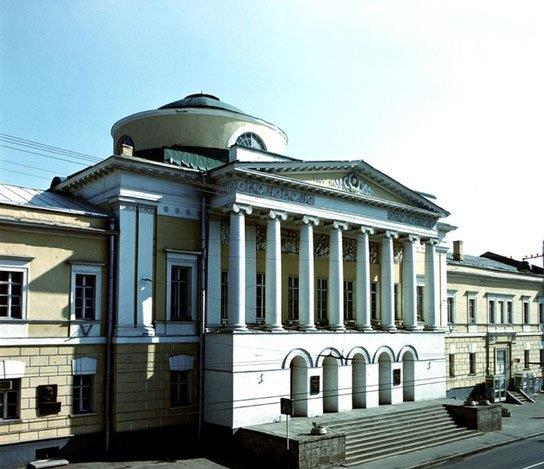
\includegraphics[width=\paperwidth - 8.5cm]{05_rsf-building}
	\end{center}
\end{wrapfigure}

To achieve its goals, the Foundation selects science and technology programs and projects that fall under certain propriety categories, and does so on a competitive basis. Among these priorities are basic research initiatives by research groups or individual scientists, or members of the higher education teaching staff; development of scientific organizations and institutions of higher education, creation of world-class departments and laboratories in scientific organizations and educational institutions, development of experimental facilities for scientific research.

The governance structure of the Foundation is set up by the Federal Law: Supervisory Board, Management board and Director General. The Federal Law sets out a  procedure for formation of these bodies as well as defines their authority. In order to provide the Foundation with the necessary expertise, the Federal law provides for creation of Review Panels acting as advisory bodies of the Foundation. Control over financial and economic activities of the Foundation is exercised by the Audit Committee of the Foundation. In accordance with the Federal Law, Russian Science Foundation submits the annual report for consideration of the President of the Russian Federation and the Government of the Russian Federation.

\vfill

\paragraph{Co-organizers}
	\begin{itemize}
		\item National Research Nuclear University MEPhI
		\item BICA Society
		\item Russian Association for Artificial Intelligence
		\item Institute for Cyber Intelligence Systems
		\item Whole Brain Architecture Initiative
	\end{itemize}

\section{Core Organizing Committee}

\subsection{General Chair}
	Alexei V. Samsonovich (George Mason University, USA; MEPhI, Moscow)

\subsection{Co-Chair}
	Valentin V. Klimov (MEPhI, Moscow)

\subsection{Committee Members}
	\begin{itemize}
		\item Aleksandr Panov (FRC CSC, Russia)
		\item Antonio Chella (University of Palermo, Italy)
		\item Michele Ferrante (Boston University, USA)
		\item Kamilla R. Jóhannsdóttir (Reykjavik University, Iceland)
		\item Olivier Georgeon (Universite Claude Bernard Lyon, France)
		\item Christian Lebiere (CMU, USA)
		\item Paul Robertson (DOLL, Inc., USA)
		\item Terry C. Stewart (U.Waterloo, Canada)
	\end{itemize}
	
\subsection{Program Committee Chairs}
	\begin{itemize}
		\item Alexei V. Samsonovich (George Mason University, USA; MEPhI, Moscow)
		\item Valentin V. Klimov (MEPhI, Moscow)
	\end{itemize}


\subsection{Program Committee Members}
	\begin{multicols}{2}
		\begin{itemize}
			\item Kenji Araki
			\item Joscha Bach
			\item Paul Baxter
			\item Paul Benjamin
			\item Tarek Besold
			\item Jordi Bieger
			\item Perrin Bignoli
			\item Douglas Blank
			\item Mikhail Burtsev
			\item Erik Cambria
			\item Suhas Chelian
			\item Antonio Chella
			\item Amelie Cordier
			\item Christopher Dancy
			\item Haris Dindo
			\item Sergey Dolenko
			\item Jim Eilbert
			\item Thomas Eskridge
			\item Usef Faghihi
			\item Stanley Franklin
			\item Herve Frezza-Buet
			\item Salvatore Gaglio
			\item Olivier Georgeon
			\item Ian Horswill
			\item Eva Hudlicka
			\item Christian Huyck
			\item Ignazio Infantino
			\item Eduardo Izquierdo
			\item Alex James
			\item Li Jinhai
			\item Magnus Johnsson
			\item Darsana Josyula
			\item Kamilla Jóhannsdóttir
			\item William Kennedy
			\item Deepak Khosla
			\item Giuseppe La Tona
			\item Luis Lamb
			\item Othalia Larue
			\item Christian Lebiere
			\item Jürgen Leitner
			\item Simon Levy
			\item Antonio Lieto
			\item James Marshall
			\item Steve Morphet
			\item Amitabha Mukerjee
			\item David Noelle
			\item Andrea Omicini
			\item David Peebles
			\item Giovanni Pilato
			\item Michal Ptaszynski
			\item Subramanian Ramamoorthy
			\item Uma Ramamurthy
			\item Thomas Recchia
			\item Vladimir Redko
			\item James Reggia
			\item Frank Ritter
			\item Paul Robertson
			\item Brandon Rohrer
			\item Paul Rosenbloom
			\item Christopher Rouff
			\item Rafal Rzepka
			\item Swathikiran S.
			\item Ilias Sakellariou
			\item Fredrik Sandin
			\item Ricardo Sanz
			\item Michael Schader
			\item Michael Schoelles
			\item Valeria Seidita
			\item Ignacio Serrano
			\item Javier Snaider
			\item Donald Sofge
			\item Rosario Sorbello
			\item Terry Stewart
			\item Sherin Sugathan
			\item Junichi Takeno
			\item Knud Thomsen
			\item Rodrigo Ventura
			\item Pei Wang
			\item Mark Waser
			\item Tom Ziemke
		\end{itemize}
	\end{multicols}

%----------------------------------------------------------------------------------------
%	CHAPTER 6
%----------------------------------------------------------------------------------------

\chapterimage{06_head_abstracts_lectures}

\chapter{Lectures, Keynotes and Talks}

\begin{enumerate}
	
	
	\paperabstract
	{Cynthia Avila-Contreras, Felix Ramos, Daniel Madrigal and Juan Luis Del Valle-Padilla}
	{A bioinspired model of early visual processing with feature and space based saliency for a cognitive architecture}
	{2017-08-05, 08:00}
	{We present a computational model that describes the early stages of visual processing and the within selective attention mechanisms to generate feature-based (hue or color) activations of salient localizations based on neurophysiology evidence of selective responses in the visual pathway. The model identifies related brain areas, the feasible computations of each one, and proposes the type of data generated and shared among the components. This work is part of the selective aspect of an attention system designed for a broader cognitive architecture for virtual creatures.}
	
	
	\paperabstract
	{Umberto Maniscalco}
	{A Bio-Ispired Aritifcial Somatosensory System for a Humanoid Robot}
	{2017-08-01, 11:15}
	{}
	
	
	\paperabstract
	{Ryutaro Ichise}
	{A Cognitive Architecture Consisting of Human Intelligence Factors}
	{2017-08-04, 12:00}
	{While there are many types of cognitive architectures available today, one thing common to all of them is the need to cover the maximum number of the human intelligence factors used for solving various tasks. However, the currently existing cognitive architectures were developed based on a variety of aspects other than the human intelligence factors. One famous model of human intelligence factors is the CHC model which is studied in psychology.When it is used as the basis of a new cognitive architecture,the architecture will cover all the known human intelligent factors used for solving various tasks. In this paper, we propose a new cognitive architecture for dialogue situations based on the CHC model as the first step towards the formation of a comprehensive cognitive architecture. We will also outline the initial architecture using a case study.}
	
	
	\paperabstract
	{Yuichi Takayama and Junichi Takeno}
	{A conscious robot that can venture into an unknown environment in search of pleasure}
	{2017-08-04, 10:30}
	{A conscious system that can venture into an unknown environment has been proposed. This study models the process of consciousness of a person who is going into an unknown environment. First, we assumed that to go into an unknown environment, the person needs to be curious about that environment and assured of its safety. Curiosity is a tendency to become interested in unknown phenomena and draw information from them. We consider that to acquire the behavior of going into an unknown environment (curiosity behavior), firstly the person needs in some way to go through many experiences of pleasure in unknown environments and increase curiosity and interest in such environments. To enter an unknown environment the person must also be assured that the environment is safe. We have developed a conscious system that can venture into an unknown environment and tested whether a robot can voluntarily enter an unknown environment.}
	
	
	\paperabstract
	{Ricardo Gudwin}
	{A Hands-on Laboratory Tutorial on Using CST to build a Cognitive Architecture}
	{01.08.2017, 10:00}
	{In this tutorial laboratory, we provide a step-by-step set of programming experiments illustrating the main foundations of the CST Cognitive Systems Toolkit in building a cognitive architecture to work as an artificial mind for controlling an NPC (non-player character) in a 3D virtual environment computer game. We start by understanding the sensors and actuators available in the NPC and how to control it inside the game. Then, we introduce the main foundations of CST: Codelets and Memories, and how they should be used to integrate a cognitive architecture. Then, we start building specific codelets and memories for a simple instance of the CST Reference Cognitive Architcture and start using it to control the NPC. The lab is a hand-on programming lab, using Java and Netbeans as language/tool. The attendant should be proficient in programming in Java language in order to follow the tutorial.    The headlines of the tutorial can be seen at: http://cst.fee.unicamp.br/tutorials}
	
	
	\paperabstract
	{Thomas Collins and Wei-Min Shen}
	{A Robust Cognitive Architecture for Learning from Surprises}
	{2017-08-03, 09:00}
	{Learning from surprises is a cornerstone for building bio-inspired cognitive architectures that can autonomously learn from interactions with their environments. However, distinguishing true surprises -- from which useful information can be extracted to improve an agents world model -- from environmental noise arising from uncertainty is a fundamental challenge. This paper proposes a new and robust approach for actively learning a predictive model of discrete, stochastic, partially-observable environments  based on a concept called the Stochastic Distinguishing Experiment (SDE). SDEs are conditional probability distributions over the next observation given a variable-length sequence of ordered actions and expected observations up to the present that partition the space of possible agent histories, thus forming an approximate predictive representation of state. We derive this SDE-based learning algorithm and present theoretical proofs of its convergence and computational complexity. Theoretical and experimental results in small environments with important theoretical properties demonstrate the algorithms ability to build an accurate predictive model from one continuous interaction with its environment without requiring any prior knowledge of the underlying state space, the number of SDEs to use or even a bound on SDE length.}
	
	
	\paperabstract
	{Gennady Osipov}
	{A sign-based model of the world and planning of collective activity}
	{2017-08-01, 17:15}
	{Sign-based formalism is considered. The concept of sign arose in the framework of semiotics. Neurophysiological and psychological researches indicate sign-based structures, which are the basic elements of the world model of a human subject.  In this formalism it was possible to formulate and solve some problems of behavior modeling, in particular, generating the goal of behavior and dynamic distribution of roles in coalition of actors.}
	
	
	\paperabstract
	{Anna Epishkina and Sergey Zapechnikov}
	{A technique of blockchain dispersal for efficient storage}
	{2017-08-01, 14:30}
	{Blockchain has become a very popular technique of creating non-editable data registers. Over time, very significant amount of data accumulates in these registers. At the same time access to this data occurs relatively rarely, mainly in order to take reference or resolve conflicts. Traditional technology implies that each participant of peer-to-peer network stores a full copy of the blockchain. We propose to apply algorithms of information array dispersal and reconstruction to drastically reduce the amount of data stored by nodes of blockchain network. We provide evaluation of memory usage efficiency to store the blockchain using these methods.}
	
	
	\paperabstract
	{Daniil A. Azarnov, Arthur A. Chubarov and Alexei V. Samsonovich}
	{A Virtual Actor with Social-Emotional Intelligence}
	{2017-08-04, 15:15}
	{This work continues the effort to design and test a universal cognitive model of emotionally biased behavior control and decision making, with the focus on social emotional relationships. Two key building blocks of the model include (i) dynamics of mutual appraisals of actors, determining the likelihoods of action selection, and (ii) moral schemas, or M-schemas, that establish normal behavior of two actors with respect to each other as well as to other entities, under certain implicit mutual relationships, such as partnership. To test the model, we implement a virtual actor embodied as an avatar in a specifically designed virtual environment, and use several paradigms of social interaction. Virtual environments and associated paradigms can be divided into a hierarchy, on top of which are paradigms with dynamically changing social relationships and roles. Using paradigms of this kind, we show that a virtual actor can be indistinguishable from a human participant, both, in its believability and in social acceptability; the latter being measured by the frequency of obtaining help from others. A model of this sort is expected to have broad applications in various fields in the near future.}
	
	
	\paperabstract
	{Evgenii Vityaev and Alexander Demin}
	{Adaptive control of modular robots}
	{2017-08-03, 08:30}
	{This paper proposes a learning control system of modular systems with a large number of degrees of freedom based on joint learning of modules, starting with finding the common control rules for all modules and finishing with their subsequent specification in accordance with the ideas of the semantic probabilistic inference. With an interactive 3D simulator, a number of successful experiments were carried out to train three robot models: snake-like robot, multiped robot and trunk-like robot. Pilot studies have shown that the approach proposed is quite effective and can be used to control the complex modular systems with many degrees of freedom.}
	
	
	\paperabstract
	{Mikhail Kupriyashin and Georgii Borzunov}
	{Algorithmic Foundation for Benchmarking of Computational Platforms Running Asymmetric Cryptosystems}
	{2017-08-01, 11:30}
	{General purpose benchmarks do not yield accurate performance estimates for special tasks. In this paper we consider implementation of exact algorithms for the 0-1 Knapsack Problem in order to determine the performance of parallel computation platforms intended for running or performing analysis on asymmetric ciphersystems. We study some features of exact parallel algorithms for the Knapsack Problem, as well as load balancing techniques for them. We propose an algorithmic foundation for computational platform benchmarking aimed at getting accurate performance estimates for these platforms.}
	
	
	\paperabstract
	{Rosario Sorbello, Salvatore Tramonte, Carmelo Calo, Marcello Giardina, Shuichi Nishio, Hiroshi Ishiguro and Antonio Chella}
	{An Android Architecture for Bio-inspired Honest Signalling in Human-Humanoid Interaction}
	{2017-08-05, 15:30}
	{This paper outlines an augmented robotic architecture to study the conditions of successful Human-Humanoid Interaction (HHI). The architecture is designed as a testable model generator for interaction centred on the ability to emit, display and detect honest signals. First we overview the biological theory in which the concept of honest signals has been put forward in order to assess its explanatory power. We reconstruct the application of the concept of honest signalling in accounting for interaction in strategic contexts and in laying bare the foundation for an automated social metrics. We describe the modules of the architecture, which is intended to implement the concept of honest signalling in connection with a refinement provided by delivering the sense of co-presence in a shared environment. Finally, an analysis of Honest Signals, in term of body postures, exhibited by participants during the preliminary experiment with the Geminoid Hi-1 is provided.}
	
	
	\paperabstract
	{Natalia Miloslavskaya}
	{Analysis of SIEM Systems and their Usage in Security Operations and Security Intelligence Centers}
	{2017-08-01, 16:30}
	{To achieve business objectives, to stay competitive and to operate legally modern organizations of all types (e.g. commercial enterprises, government agencies, not-for profit organizations), different size and sphere of activity need to match a lot of internal and external requirements. They are called compliance regulations and mean conforming to a rule, such as a specification, procedure, policy, standard, law, etc. These organizations need to ensure valuable assets, uninterrupted business operation (processes), reliable data and differentiated quality of service (QoS) to various groups of users. They need to protect their clients and employees not only inside but also outside organization itself in connection with which two new terms were introduced - teleworking or telecommuting. According to Gartner by 2020, 30\% of global enterprises will have been directly compromised by an independent group of cybercriminals or cyberactivists. And in 60\% of network breaches, hackers compromise the network within minutes, says Verizon in the 2015 Data Breach Investigations Report. An integrated system to manage organizations intranet security is required as never before. The data collected and analyzed within this system should be evaluated online from a viewpoint of any information security (IS) incident to find its source, consider its type, weight its consequences, visualize its vector, associate all target systems, prioritize countermeasures and offer mitigation solutions with weighted impact relevance. The brief analysis of a concept and evolution of Security Information and Event Management (SIEM) systems and their usage in Security Operations Centers and Security Intelligence Centers for intranets IS management are presented.}
		
		
		\paperabstract
		{Dmitry Filin and Aleksandr I. Panov}
		{Applying a neural network architecture with spatio-temporal connections to the maze exploration}
		{2017-08-02, 14:45}
		{We present a model of Reinforcement Learning, which consists of modified neural-network architecture with spatio-temporal connections, known as Temporal Hebbian Self-Organizing Map (THSOM). A number of experiments were conducted to test the model on the maze solving problem. The algorithm demonstrates sustainable learning, building a near to optimal routes. This work describe nan agents behavior in the mazes of different complexity and also influence of models parameters at the length of formed paths.}
		
		
		\paperabstract
		{Anton Kolonin}
		{Architecture of Internet Agent with Social Awareness}
		{2017-08-04, 17:30}
		{We describe approach, architecture, implementation and practical applications of personal software agent with social awareness, capable to capture socio-temporal context of its user on the Web and in social networks in the course of interactions of the user with agent itself and user's Internet environments online.}
		
		
		\paperabstract
		{Olivier Georgeon}
		{Artificial lifelong incremental learning: a gentle start}
		{2017-08-01, 14:00}
		{The challenge of designing robots that can learn incremental sensorimotor skills from their autonomous experience interacting with the world throughout their life has gained increasing interest recently. For example, the European commission just funded the Goal-Robot project to address this challenge. Cognitive theories suggest that such incremental sensorimotor learning could pave the way to higher-level intelligence. However, we are still missing a unified theory of developmental learning to solve this challenge. Indeed, current research on artificial developmental learning mostly focuses on specific developmental steps instead of lifelong developmental principles. I will present a new hierarchical sequence learning algorithm and show how it can help make progress addressing this challenge.  The main principle learned is to refer to the robots sensor data as feedback from the robots actions as opposed to passive perception of a pre-given world.}
		
		
		\paperabstract
		{Rosario Sorbello, Salvatore Tramonte, Marcello Giardina, Carmelo Cali, Shuichi Nishio, Hiroshi Ishiguro and Antonio Chella}
		{Augmented Embodied Emotions by Geminoid Robot induced by Human Bio-feedback Brain Features in a Musical Experience}
		{2017-08-02, 14:45}
		{This paper presents the conceptual framework for a study of musical experience and the associated architecture centred on Human-Humanoid Interaction (HHI). We discuss the state of the art of the theoretical and the experimental research into the cognitive capacity of music. We overview the results that points  to the correspondence between the perceptual structures, the cognitive organization of sounds in music, the motor and affective behaviour. On such grounds we bring in the concepts of musical tensions and functional connections as the constructs that account for such correspondence in music experience. Finally we describe the architecture as a models generator system whose  modules can be employed to test this correspondence from which the perceptual, cognitive, affective and motor constituents of musical capacity may emerge.}
		
		
		\paperabstract
		{Jonathan Rosales, Myrna S. Zamarripa, Felix Ramos and Marco-Antonio Ramos}
		{Automatic reward system for virtual creatures, emergent processes of emotions and physiological motivation}
		{2017-08-05, 12:00}
		{Emotional and motivational evaluations are part of the development of rewards within living beings. Particularly, during the perception of stimuli in the environment, these evaluations collaborate with one another to generate reward values automatically, without the need to involve rational processes. In this paper we propose a conceptual model of automatic reward for virtual creatures inspired by neuroscientific evidence, contemplating the processes of emotions and motivations, as well as the generation and recovery of automatic reward values. According to the evidence, the reward process is divided into two processes: liking, which is oriented toward interpreting information inputs and generating reward values, and wanting, focused on the recovery of the stored reward values and the generation of objectives in the environment. The reward process is implemented as a concurrent and parallel naturally distributed system, allowing virtual creatures to adapt to their environment and generate more credible behaviors. The results of liking and wanting are shown in this article through a case study, in which the performance of both processes is observed when the creature interacts with the environment.}
		
		
		\paperabstract
		{Alexei V. Samsonovich}
		{Biologically Inspired Cognitive Architectures: An introduction}
		{2017-08-01, 08:15}
		{}
		
		
		\paperabstract
		{Evgenii Vityaev and Alexander Demin}
		{Cognitive architecture based on the functional systems theory}
		{2017-08-05, 11:00}
		{In this paper the cognitive architecture based on the Functional Systems Theory (TFS) by P.K.Anokhin is presented. This architecture based on the main notions of this theory: goal, result, anticipation of the result. This theory is described on physiological and informational level. The logical structure of this theory was analyzed and used for the control system of the purposeful behavior development. This control system contains the hierarchy of functional systems that organize the purposeful behavior. The control system was used for the agents modeling that are solving the foraging task. The computer experiments are presented that compare this control system with the control systems based on the reinforcement learning.}
		
		
		\paperabstract
		{Ignazio Infantino}
		{Computational Creativity for Cognitive Robots}
		{2017-08-01, 09:00}
		{}
		
		
		\paperabstract
		{Hidemoto Nakada and Yuuji Ichisugi Ichisugi}
		{Context-Dependent Robust Text Recognition using Large-scale Restricted Bayesian Network}
		{2017-08-04, 15:30}
		{We have been proposing a computational model of the cerebral cor- tex called BESOM, which models the cerebral cortex as restricted Bayesian net- works based on recent findings in the neuroscience area. Since BESOM is based on Bayesian network, it inherently allows bi-directional information flow, meaning that it can naturally merge information extracted from concrete data with highly- abstract prior knowledge. As an example of such kind of tasks, we report robust text recognition task with context information. We show that word spelling knowledge and word n-gram could be represented as a part of the network and actually they contribute the text recognition accuracy with noisy text images. We also show that the computational cost is approximately linear with the number of characters and words.}
		
		
		\paperabstract
		{Paul Robertson and Robert Laddaga}
		{Context-driven Active-sensing for Repair Tasks}
		{2017-08-03, 16:30}
		{The CART project aims to enable robotic helpers for repair mission the use models of repair missions, to guide active perception in supporting the understanding of the steps being taken by a human operator and to offer assistance in a timely manner based on story understanding.}
		
		
		\paperabstract
		{Oleg Nikitin and Olga Lukyanova}
		{Control of an agent in the multi-goal environment with homeostasis-based neural network}
		{2017-08-04, 14:00}
		{Here we present the model of bio-inspired neuron, and synaptic plasticity, incorporating cellular homeostasis. Network of such neurons is used for multi-goal oriented control task. It was showed that such a model provides adaptive and robust behavior for the controlled agent.}
		
		
		\paperabstract
		{Nikita Ushakov and Vitaliy Ivanenko}
		{Copyright protection of video content based on digital watermarks}
		{2017-08-01, 12:00}
		{The paper proposes the method of digital watermark usage for video copyright protection, that may be a solution to the piracy of digital content. This paper studies different watermark embedding methods for videos. Modified DEW watermarking algorithm is proposed. This method stands out for its technique - the watermark is embedded exclusively by discarding certain high frequency coefficients. Different attacks on video container were studied. The watermark was exposed to most of the common attacks. Performance factors of this algorithm were calculated, they depend on three parameters: energy difference, cut-off point and the number of DCT blocks. Effective values of the parameters were found. The suggested method may act as an effective option for copyright protection.}
		
		
		\paperabstract
		{Aleksander Boruchinkin, Anastasia Tolstaya and Arseniy Zhgilev}
		{Cryptographic Wireless Communication Device}
		{2017-08-02, 09:30}
		{The total increase in the use of mobile devices inevitably leads to an increase in the number of different security threats. The cryptographic device described in this article provides a secure (encrypted) transmission of data. It alerts the user if the crypto headset at the opposite end of the link is not trusted, thus extending the offending model (i.e. a list of the potential opportunities of the offender) to the possibility of to the possibility of substituting one of the encrypting devices. All functions for encryption and decryption are enclosed in a separate unit that connects to the phone via Bluetooth. The crypto headset specifications were compared with the closest analogues and ensures a higher level of security for each group of consumers: the corporate sector, government agencies, and individual users.}
		
		
		\paperabstract
		{Giovanni Pilato and Ernesto DAvanzo}
		{Data-driven Social Mood Analysis through the Conceptualization of Emotional Fingerprints}
		{2017-08-02, 14:00}
		{A body of knowledge shows the emerging of an evidence according to a better account for the emotion spectrum is achievable by employing a detailed selection of emotion keywords. Basic emotions, such as Ekman's ones, cannot be considered universal, but are related to with implicit thematic affairs within the corpus under analysis. The paper tracks some preliminary experiments obtained employing a data-driven methodology that captures emotions, relying on domain data that you want to model. The experimentation consists of investigating the corresponding conceptual space based on a set of terms (i.e., keywords) that are representative of the domain and the determination. Furthermore, the conceptual space is exploited as a bridge between the textual content and its sub-symbolic mapping as an ``emotional fingerprint'' into a six dimensional hyperspace.}
		
		
		\paperabstract
		{Aaron Sloman}
		{Deep, largely unnoticed, gaps in current AI, and what Alan Turing might have done about them.}
		{2017-08-03, 11:30}
		{Gaps at present include the inability of current AI systems to make discoveries made by Euclid, Archimedesw1 and other ancient mathematicians, including discoveries in geometry and topology, long before the development of modern logic, algebra, formal logic, and proof theory. The information-processing abilities required seem to be closely related to the abilities of pre-verbal human toddlers to make proto-mathematical discoveries including topological discoveries, and also forms of intelligence in nest-building birds, squirrels, elephants, orangutans and other species. Current AI vision systems cannot support the uses of vision in discovery of deep mathematical features of geometry and topology, including discovery of impossibilities and necessary connections (related to but different from perception of positive and negative action-affordances). They also lack the meta-cognitive, reflective abilities required to organise, communicate and defend such discoveries if challenged -- precursors to mathematical proof. Current AI language *learning* mechanisms cannot match the language *creating* mechanisms used by young humans, demonstrated dramatically by deaf children in Nicaragua. (See https://www.youtube.com/watch?v=pjtioIFuNf8) Current AI models of emotion and motivation support only shallow mimicry of affective states: they lack the depth and variety of biological mechanisms involved in passionate interest in mathematics, long term grief, deep patriotism, finding something hilariously funny, and many other short and long term states and processes relating to things cared about. The CogAff project attempts to address some of these issues. (http://www.cs.bham.ac.uk/research/projects/cogaff/) This is very different from, and much more difficult than, producing machines with shallow mimicry of human responses. Moreover, emphasis on embodied cognition, enactivism, and situated cognition, focuses on real but shallow products of evolution, ignoring requirements for increasingly *disembodied* forms of cognition to meet increasingly complex and varied challenges in sophisticated organisms inhabiting complex, extended, multi-faceted terrain. The emphasis on embodiment also ignores requirements to apply meta-cognitive processes to oneself and to others, and abilities to invent, implement, test, debug, and modify novel and increasingly complex engineering solutions to practical problems. Designers of ancient pyramids could not plan a new creation by physically interacting with the materials tools, labourers and temporary structures used during construction. It is likely that the vast majority of important evolutionary transitions in information processing, and the products in animal brains, have not yet been discovered, and that some of them cannot be detected by current scanning mechanisms (which don  reveal subneural processes, e.g. the chemistry of a synapse). Inspired by a conjecture about what Turing might have worked on if he had not died two years after publishing his paper on morphogenesis, the tutorial will present the conjectured roles of both the fundamental construction kit provided by physics and chemistry and multiple derived construction kits produced by evolution, often straddling different species. Without the later construction kits, current species could not exist. Some of the construction-kits are required mainly for physical (physiological) structures. Others are required for construction of new forms of information processing. There may be important examples that human scientists have not yet (re-)discovered.}
		
		
		\paperabstract
		{Mikhail Alyushin and Lyubov Kolobashkina}
		{Development of a Metrological Database with Images  of a Human Face in the Infrared Range to Evaluate  the Effectiveness of Biometric Algorithms}
		{2017-08-04, 09:00}
		{The work shows the promise of using biometric algorithms intended for remote determination of current human bio-parameters based on processing of the infrared image of his face. Problems that hinder the widespread use of remote biometric algorithms in practice are highlighted. The urgency of creating a metrological database containing video recordings of the human face image in the infrared range for the evaluation of the biometric algorithms efficiency is substantiated. Presented are the results of an analysis of existing databases containing images of a persons face. Insufficient development of specialized databases containing infrared images of a persons face was noted. The main shortcomings of such databases are highlighted. An approach to creating a metrological database based on the acquisition and storage of complex personal data is proposed. The main components of such data are video recordings of the face image in the visible and infrared ranges, time synchronized records of human bio-parameters, as well as information on the complexity of test tasks performed. The structure of the laboratory system for obtaining complex data on the person undergoing testing is considered. A typical data structure for a single test cycle is presented. The application results of the first version of the metrological database for experimental research of the effectiveness of algorithms for remote determination of human bio-parameters are presented.}
		
		
		\paperabstract
		{Anna Epishkina and Sergey Zapechnikov}
		{Discovering and clustering hidden time patterns in blockchain ledger}
		{2017-08-01, 15:00}
		{Currently, non-editable blockchain-based ledgers become important tools for cryptocurrency transactions, auditing, smart contracts, copyright registration and many other applications. In this regard, there is a need to analyze the typical, repetitive actions written to the ledger, for example, to identify suspicious cryptocurrency transactions, a chain of events that led to information security incident, or to predict recurrence of some situation in the future. We propose to use for these purposes the algorithms for T-patterns discovering and to cluster the identified behavioral patterns subsequently. In case of having labeled patterns, clustering might be replaced by classification.}
		
		
		\paperabstract
		{Tomoya Sumioka and Junichi Takeno}
		{Discussion of Stalking Behavior Using a Conscious System}
		{2017-08-04, 09:30}
		{Stalking behavior, characterized by specific and dreadful acts such as persistent following, repeated sending of unwanted gifts, lack of sympathy, and even willingness to kill the victim, has become a serious concern in modern society. However, since stalking behavior has something partly in common with any criminal behavior, further discussion of this topic is considered helpful in determining factors behind various criminal behavior. Thus, there is an urgent need to investigate how this mysterious and dangerous behavior arises. There are three main types of stalking behavior: ``rejected,'' ``resentful,'' and ``other (intimacy seeker and incompetent suitor).'' First, we focused on a conscious model of the rejected type, as it is considered the most typical. The artificial conscious model is built to represent a process in which a conflict of concepts arising in the Reason Subsystem is progressively reconciled by the Association Subsystem.}
		
		
		\paperabstract
		{Soichiro Arai and Junichi Takeno}
		{Discussion on explicit consciousness, sub-consciousness, and self-awareness in a conscious system}
		{2017-08-04, 16:30}
		{What is ``self-awareness''? How can explicit consciousness and sub-consciousness be mapped in relation to each other? How are they related to the self? How can these entities be represented in an artificial conscious system? These questions are the focus of this article. People are aware of only the behavior that they are focusing on; they cannot be directly aware of routine behavior such as walking and breathing. The latter is generally called unconscious behavior, and here we call it sub-conscious behavior. To understand self-awareness, therefore, firstly it is important to map explicit consciousness and sub-consciousness, which is where the self is deeply involved. We consider that if there is no self that refers to itself, no one can be aware of what he himself is doing. In this study we map explicit consciousness and sub-consciousness using an artificial conscious system, and then make a new proposal about the relationship between self-awareness and the self.}
		
		
		\paperabstract
		{Kensuke Arai and Junichi Takeno}
		{Discussion on the Rise of the Self in a Conscious System}
		{2017-08-04, 08:30}
		{What is human self? Some argue that there is no such thing as self. However, the subjective feeling that ``I am writing these words'' makes it hard to deny the existence of the self. We assume that as long as there is the term ``self,'' there must be some collection of neural networks that represents the concept of the term. Although the whole picture is still a mystery, we have taken a step forward to unraveling the mystery by introducing the idea that ``the emergence of a new behavior that prioritizes the body underlies the rise of the self.'' When performing imitation behavior, a person can encounter a situation in which he feels pain and tries to avoid it. In this instance, the person engages in two types of behavior almost simultaneously, which are in conflict with each other. Also in this instance, it is assumed that the person gives priority to the safety of his own body and reflexively chooses to respond with avoidance behavior. However, as the imitation behavior continues, the process of imitation and avoidance is repeated many times, making it increasingly difficult to ensure the safety of the body. To address this scenario, we have come up with an idea that enables a conscious system to generate a new rational behaviorthat is, voluntarily stop the imitation behavior. We consider that the generation of this new behavior is a significant process that can explain the first step for the development of the self.}
		
		
		\paperabstract
		{Victor Morozov and Natalia Miloslavskaya}
		{DLP Systems as a Modern Information Security Control}
		{2017-08-01, 17:45}
		{Today, information is one of the most critical and valuable assets for success and prosperity of any company. The complexity of modern organizations and the trend to move to the cloud and outsource are increasing. At the same time the wide range of new ever-growing information security (IS) threats, especially those related to new information, communication and network technologies, services and devices, are all around us. For example, the well-publicized attack on the Sony Playstation Network, resulted in the loss of user names, passwords, ad-dresses, birth dates and financial details of 77 million users and Sony's financial loss around \$171 million (including estimates for customer support costs, legal costs and the impact on future profits), left the online gaming network suspended for weeks in 2011. The importance of using modern protection tools against inter-nal IS threats is proved. The advantages of DLP systems over alternative solutions are disclosed. The principles and technologies underlying the operation of DLP systems are discussed. The architecture, application features and analytical capabilities of the SearchInform Information Security Perimeter (SearchInform) DLP system are described in detail.}
		
		
		\paperabstract
		{Kazuteru Miyazaki}
		{Exploitation-Oriented Learning with Deep Learning   -Comparison with a Deep Q-network-}
		{2017-08-04, 17:00}
		{Deep learning has attracted significant interest currently. The deep Q-network (DQN) combined with Q-learning have demonstrated excellent results for several Atari 2600 games. In this paper, we propose an exploitation-oriented learning (XoL) method that incorporates deep learning to reduce the number of trial-and-error searches. We focus on a profit sharing (PS) method that is an XoL method and combine a DQN and PS. The proposed method DQNwithPS is compared to a DQN in Pong of Atari 2600 games. We demonstrate that the proposed DQNwithPS method can learn stably with fewer trial-and-error searches than only using a DQN.}
		
		
		\paperabstract
		{Andrey Trukhachev and Natalia Ivanova}
		{Extracting of High-level Structural Representation from VLSI Circuit Description Using Tangled Logic Structures}
		{2017-08-02, 08:00}
		{This paper proposes a method of automatic VLSI circuit analysis. On the first step transistors are grouped by their structure. Groups with irregular structure are highly interconnected to each other. Detecting Tangled Logic Structures (TLS) with a GTL-depended linear ordering and genetic algorithm divides the circuit due to its functional structure and forms the gate-level VLSI circuit.  High-level functional blocks in circuit description consist of gate-level cells groups, which are also highly interconnected. After TLS-blocks extracting, it is possible to describe their function. TLS-blocks are smaller, represent a cell of high-level circuit, and are thus more suitable for further functional circuit analysis than a gate-level VLSI circuit.}
		
		
		\paperabstract
		{Yury Prostov and Yury Tiumentsev}
		{Functional Plasticity in a Recurrent Neurodynamic Model: from Gradual to Trigger Behavior}
		{2017-08-05, 11:00}
		{Dynamic model of a recurrent neuron with sigmoidal activation function is considered. It is shown that the neuron activation characteristic (dependence between an input pattern and an output signal) can have the form of both a smooth sigmoidal function and a step function in the form of a quasi-rectangular hysteresis loop due to the presence of the modulation parameter. We demonstrate that a gradual behaviour in the network can be implemented which means that neurons will have output values proportional to how each of them corresponds to the input pattern. In this case signals in the network will be propagated freely but with attenuation. The output values of the neurons also will be low. At the same time a winner-takes-all behaviour can be implemented which means that neurons becomes similar to threshold units. As a result, there will be limited network activity since only a part of the neurons will have output values close to the maximum value while the remaining neurons will have output values close to the minimum value. Thus the presence of the modulation parameter provides a means to change quickly the behavior strategy of the network which affects the processes of pattern recognition and learning.}
		
		
		\paperabstract
		{Aleksandr I. Panov, Konstantin S. Yakovlev and Roman Suvorov}
		{Grid Path Planning with Deep Reinforcement Learning: Preliminary Results}
		{2017-08-05, 08:30}
		{Single-shot grid-based path finding is an important problem with the applications in robotics, video games etc. Typically in AI community heuristic search methods (based on A* and its variations) are used to solve it. In this work we present the results of preliminary studies on how neural networks can be utilized to path planning on square grids, e.g. how well they can cope with path finding tasks by themselves as well as how they can be put into service to the conventional heuristic search algorithms, e.g. A*. Conducted experiments show that the agent robustly learns to achieve the goal and that the adaptive heuristic is capable of reducing breadth of the search tree.}
		
		
		\paperabstract
		{Anastasia Beresneva, Anna Epishkina, Sergey Babkin, Alexey Kurnev and Vladimir Lermontov}
		{Handwritten Signature Verification: the State of The Art}
		{2017-08-01, 11:00}
		{Nowadays handwritten signature and its verification is utilized in a lot of applications including e-commerce. An analysis of verification algorithms and areas of their practical usage is provided. The focus of the investigation is on verification method based on neural network. This type of verification algorithm is realized as a mobile application and its main characteristics are obtained. The directions of further work are concluded including a modification of an algorithm and its realization in order to remove its disadvantages.}
		
		
		\paperabstract
		{Christian Tsvetkov and Ivan Vankov}
		{How do deep neural networks represent faces?}
		{2017-08-05, 10:30}
		{Deep learning models of vision have recently achieved human-level of performance in tasks such as object recognition and face identification. However, the extent to which these computational models resemble the way biological vision works remains unclear. We address this question by investigating how a deep learning model of face identification represents faces and by comparing the results to data from behavioural experiments. To this end, we use the Bubbles technique (Gosselin \& Schyns, 2001) in order to find the critical regions within an image which are needed for correct face identification. The technique is applied to a pretrained deep convolutional neural network model of face recognition (Amos, Ludwiczuk, \& Satyanarayanan, 2016), and the results are related to human data from a replication of Gosselin \& Schyns (2001). We also use Bubbles to check how faces are represented in a simple connectionist model and in a deep learning model trained on general object recognition.}
		
		
		\paperabstract
		{David Kelley and Mark Waser}
		{Human-like Emotional Responses in a Simplified Independent Core Observer Model System}
		{2017-08-02, 15:30}
		{Most artificial general intelligence (AGI) system developers have been focused upon intelligence (the ability to achieve goals, perform tasks or solve problems) rather than motivation (*why* the system does what it does).  As a result, most AGIs have an unhuman-like, and arguably dangerous, top-down hierarchical goal structure as the sole driver of their choices and actions.  On the other hand, the independent core observer model (ICOM) was specifically designed to have a human-like ``emotional'' motivational system.  We report here on the most recent versions of and experiments upon our latest ICOM-based systems.  We have moved from a partial implementation of the abstruse and overly complex Wilcox model of emotions to a more complete implementation of the simpler Plutchik model.  We have seen responses that, at first glance, were surprising and seem-ingly illogical  but which mirror human responses and which make total sense when considered more fully in the context of surviving in the real world.  For ex-ample, in ``isolation studies'', we find that any input, even pain, is preferred over having no input at all.  We believe that the fact that the system generates such un-expected but ``humanlike'' behavior to be a very good sign that we are successful-ly capturing the essence of the only known operational motivational system.}
		
		
		\paperabstract
		{Alisa Volkert, Stefanie Mueller and Alexandra Kirsch}
		{Human-like Prototypes for Psychologically Inspired Knowledge Representation}
		{2017-08-04, 10:30}
		{We evaluate human grouping of everyday objects for a psychologically inspired knowledge representation based on prototype theory. Our overall aim is to develop a knowledge representation system that one day could be used by kitchen robots. We conducted a study in which participants had to sort different kitchen objects into a digital kitchen. We chose a kitchen as a use case, since people have to tidy up dishes every day. We calculated an overall similarity matrix and identified object groups whenever at least half of the participants put two items on the same shelf. Out of these object categories we calculated the respective prototype. We then tested the similarities of all categories to all prototypes, which turned out to be reasonable.}
		
		
		\paperabstract
		{Amit Kumar Mishra}
		{ICABiDAS: Intuition Centred Architecture for Big Data Analysis and Synthesis}
		{2017-08-01, 14:45}
		{Humans are expert in the amount of sensory data they deal with each moment. Human brain not only ``analyses'' these data but also starts ``synthesizing'' new information from the existing data. The current age Big-data systems are needed not just to analyse data but also to come up new interpretation. We believe that the pivotal ability in human brain which enables us to do this is what is known as ``intuition''. Here, we present an intuition based architecture for big data analysis and synthesis.}
		
		
		\paperabstract
		{Maksim Sharaev, Vyacheslav Orlov, Vadim Ushakov and Boris Velichkovsky}
		{Information transfer between rich-club structures in the human brain}
		{2017-08-05, 10:30}
		{The performance of the human brain depends on how effectively its distinct regions communicate, especially the regions which are more strongly connected to each other than to other regions, or so called ``rich-clubs''. The aim of the current work is to find a connectivity pattern between the three brain rich-club regions without any a priori assumptions on the underlying network architecture. Rich-clubs for the analysis were previously identified with structural MRI. Functional magnetic resonance imaging (fMRI) data from 25 healthy subjects (1000 time points from each one) was acquired and Transfer Entropy (TE) between fMRI time-series from rich-clubs was calculated. The significant results at the group level were obtained by testing against the surrogate data generated on a novel approach. We found stable causal interactions between rostral Anterior Cingulate Cortex L and Dorsal Anterior Cingulate Cortex L, dorsal Anterior Cingulate Cortex L and Paracentral Lobule R but not vice versa. Our work provides an approach to causal analysis of experimental data and demonstrates the applicability to real fMRI study.}
		
		
		\paperabstract
		{Artem Chernyshov, Anita Balandina, Anastasiya Kostkina and Valentin Klimov}
		{Intelligent search system for huge non-structured data storages with domain-based natural language interface}
		{2017-08-04, 17:00}
		{Nowadays the number of huge companies and corporations has in their disposition various non-structured texts, documents and other data. The absence of clearly defined structure of the data makes the implementation of searching queries complicated and even impossible depending on the storage size. The other problem connected with staff, which may face the problem with misunderstanding of the special query languages, knowledge of which is necessary for the execution of searching queries. To solve these problems, we propose the semantic search system, the possibilities of which include the searching index construction, for queries execution and the semantic map, which would help to clarify the queries. In this paper we are going to describe our algorithms and the architecture of the system, and also to give a comparison to analogues.}
		
		
		\paperabstract
		{Vishwanathan Mohan and Ajaz Ahmad Bhat}
		{Joint Goal Human Robot collaboration-From Remembering to Inferring}
		{2017-08-05, 09:00}
		{The ability to infer goals, consequences of one's own and others' actions is a critical desirable feature for robots to truly become our companions-thereby opening up applications in several domains. This article proposes the viewpoint that the ability to remember our own past experiences based on present context enables us to infer future consequences of both our actions/goals and observed actions/goals of the other (by analogy). In this context, a biomimetic episodic memory architecture to encode diverse learning experiences of iCub humanoid is presented. The critical feature is that partial cues from the present environment like objects perceived or observed actions of a human triggers a recall of context relevant past experiences thereby enabling the robot to infer rewarding future states and engage in cooperative goal-oriented behaviors. An assembly task jointly done by human and the iCub humanoid is used to illustrate the framework.  Link between the proposed framework and emerging results from neurosciences related to shared cortical basis for remembering, imagining and perspective taking' is discussed.}
		
		
		\paperabstract
		{Antonio Lieto}
		{Knowledge Representation in Cognitive Architectures: Current Limitations and Open Challenges}
		{2017-08-02, 10:30}
		{In this talk I will provide a focused overview of the representational assumptions developed in different cognitive architectures. In doing so I will outline the main problematic aspects of the current proposals (involving the limited size and the homogeneous typology of the encoded and processed knowledge) and I present a possible way out based on different, but complementary, research agendas.}
		
		
		\paperabstract
		{Mikhail Alyushin, Alexander Alyushin and Lyubov Kolobashkina}
		{Laboratory Approbation of a New Approach for Contrast Enhancement of Human Face Thermal Image Based on Selective Multifunction Pixel Brightness Conversion Function}
		{2017-08-04, 08:00}
		{The paper suggests a new approach to improving the contrast of the thermal image of a persons face in the deep infrared region. The approach involves the analysis and modification of the histogram of the image and is based on the use of a selective multivalued function for encoding the brightness of image pixels. The approach is focused on processing first of all thermal images of the person, containing areas with various informativeness. The implementation of the approach in practice makes it possible to improve the contrast of the face image with preservation of all informative features regardless of the level of brightness of the corresponding pixels of the image. In this case, background areas with high and low levels of exposure are compressed. The effectiveness of the proposed approach was tested in laboratory tests of the developed specialized program. For this purpose, the existing library of thermal images of people of different age and sex was used. The achieved gain in the contrast level averaged 2.5 times for the most informative areas of the face. The proposed approach is focused on the use in remote sensing systems of human bioparameters.}
		
		
		\paperabstract
		{Mikhail Alyushin, Lyubov Kolobashkina and Alexander Alyushin}
		{Laboratory Approbation of the Algorithm for Isolating Peoples Faces on a Thermal Infrared Image in the Case of their Quasi-Stationary Arrangement in a Room}
		{2017-08-04, 08:30}
		{Increasing the effectiveness of training and training sessions is possible through the implementation of so-called biological feedback. Such feedback allows the teacher, or the instructor, to continuously monitor the current psycho-emotional and functional state of the students. As a result, it becomes possible to adapt the style, pace, training mode and the volume of the material outlined, depending on the current receptivity and fatigue level of the listeners. The main element of systems that implement biological feedback in practice are remote non-contact technologies. Such technologies allow in a fully automatic mode to register the main most informative human bioparameters. Among them, in the first place are the parameters characterizing the current state of the cardiovascular system of man, his breathing system, as well as his peripheral nervous system. The bulk of information is obtained by processing in real time the thermal infrared image of a persons face. Unfortunately, existing algorithms for distinguishing a persons face have a sufficiently high computational complexity and insufficient reliability. A typical example in this regard can be a family of algorithms based on the Viola-Jones approach. The approach proposed in the work is based on taking into account additional information about the most likely location of a persons face on a thermal image. This approach is most appropriate to use in cases of quasi-stationary location of people in the room. A typical example is the location of students at the tables in the classroom. For such cases it is possible to determine the areas of the most probable location of the trainees faces, as well as the possible boundaries of their movement. Laboratory tests of the developed program on the basis of the proposed algorithm have confirmed its high productivity, as well as efficiency in identifying students faces in the classroom.}
		
		
		\paperabstract
		{Eugene Borovikov and Szilard Vajda}
		{Looking at faces in the wild}
		{2017-08-05, 11:30}
		{Recent advances in the face detection (FD) and recognition (FR) technology make it appear that the problem of face image localization and matching is essentially solved, e.g. via deep learning models using thousands of samples per face for training and validation on the available benchmark data-sets. Human vision system seems to handle face localization and matching problem differently from the modern FR systems, as humans appear to detect faces instantly even in most cluttered environments, which may be evolutionary hard-wired and experience-tuned, and often require a single view of a face to reliably distinguish it from all others. This prompted us to take a biologically inspired look at building a cognitive architecture that extensively uses artificial neural nets at the face detection stage and adapts a single image per person (SIPP) approach for face image matching.}
		
		
		\paperabstract
		{Larisa Ismailova, Viacheslav Wolfengagen, Sergey Kosikov, Irina Parfenova and Iliya Nikulin}
		{Means for ensuring compatibility of heterogeneous data models in an interactive visualization environment}
		{2017-08-02, 16:30}
		{The paper considers the problem of visualizing heterogeneous information relevant to the solution of a particular problem domain. An essential part of the task is to get the conversion of data objects doing their representation adjusted for the corresponding data model. Creation of a model of converting of data objects is offered on the basis of applicative computing systems. Achievement of flexibility requires the parametrization of the considered construction, i.e. support of dependence of a set of available methods of interpretation on parameters as which semantic characteristics of processed data appear. The methods of working with interpretation coordination tools have been partially tested when implementing various applications for informational support for the implementation of the best available technologies (BAT).}
		
		
		\paperabstract
		{Liudmila Zhilyakova}
		{Model of heterogeneous interactions among complex agents. From a neural to a social network}
		{2017-08-01, 16:30}
		{We describe a heterogeneous neural network where neurons interact by means various neurotransmitters. This feature enables exerting selective influence on neurons. We use this formalism as a basis for modeling interactions between agents in a social network in which two types of opposite activity are spreading. The main properties of agents and principles of activity spreading are defined. The classification of agents according to their parameters is represented.}
		
		
		\paperabstract
		{Vladimir RedKo}
		{Model of Interaction between Learning and Evolution}
		{2017-08-01, 11:45}
		{The lecture characterizes the following main properties of interaction be-tween learning and evolution: 1) the mechanism of the genetic assimilation, 2) the hiding effect, 3) the role of the learning load at investigated processes of learning and evolution}
		
		
		\paperabstract
		{Arthur Chubarov and Daniil Azarnov}
		{Modeling Behavior  o f Virtual Actors : A Limited Turing Test  f or Social - Emotional Intelligence}
		{2017-08-04, 15:00}
		{This  work  presents  the  design,  implementation  and study  of  (1)  a  videogame -like  virtual  environment simulator, enabling  social  interaction  of  avatars  controlled  by  human participants  and  by  virtual  actors;  (2)  a  set  of  virtual  actors with varying forms and degree of social-emotional intelligence,  based  on  the  eBICA  cognitive  architecture;  and  (3)  a  limited Turing  test  for  social-emotional  intelligence,  involving  human participants   and   virtual   actors.   The virtual   environment simulator   allows   for   various   forms   of   emotionally-laden interaction of actors immersed in it in the form of avatars,  with data  collection  characterizing  their  behavior  in  detail.  The  objective  here  is  to  compare  and  evaluate  models  of  social -emotional reasoning based on the Turing test results and other  objective   behavioral   measures,   also   taking   into   account  subjective judgment of participants. One of the long -term goals is   achieving   human-level   believability   of   socially-emotional  virtual   actors,   such   as   non-player   characters   in   games, personal   assistants,   robots,   and   other   intelligent   artifacts. Preliminary  results  indicate  importance  of  social-emotional intelligence  for  believability,  and  support  assumptions  of  the eBICA architecture.}
		
		
		\paperabstract
		{Masahiro Miyata and Takashi Omori}
		{Modeling emotion and inference as a value calculation system}
		{2017-08-04, 11:00}
		{There were many modeling studies on the emotion. But most of them were phenomenological and don't approach to the brain or cognitive mechanism. In this study, we discuss on a possibility of its computational modeling based on an idea that an emotion in a wider sense is a value calculation system for an action decision. First, we show a possible brain architecture that the emotion system has a tight interaction with the cortical intelligent system through an interaction between the brain information processing areas of neocortex and limbic system. Then, in this study, we focused on a mechanism of value based intuitive inference on a path finding task in a partially known world. In a computer simulation, we tried to make a model of brainstem that is one of the brain emotion system parts. Though the brainstem looks simple, the model includes an essence of conflict resolving between multiple values.}
		
		
		\paperabstract
		{Lubov Podladchikova, Anatoly Samarin, Dmitry Shaposhnikov and Mikhail Petrushan}
		{Modern views on visual attention mechanisms}
		{2017-08-02, 10:30}
		{Modern views on visual attention mechanisms, some results of our last psychophysical experiments with eye movements recording and future steps of studying have been considered. Several groups of finding have been determined, namely: (i) unresolved objectives; (ii) problems for which contradictory data are known; (iii) finding which propose revision of some classic views; (iv) views consistent with data obtained in different research centers. The results of psychophysical tests directed on receiving of quantitative parameters of eye movements at performance of different visual tasks to estimate the contribution of bottom-up and top-down mechanisms of visual attention are presented. It is supposed that obtained experimental results can be formalized to use in realistic mathematical models of visual attention.}
		
		
		\paperabstract
		{Dharani Punithan and Byoung-Tak Zhang}
		{Molecular Associative Memory with Spatial Auto-logistic Model for Pattern Recall}
		{2017-08-05, 11:30}
		{We propose a molecular associative memory model, by combining auto-logistic specifications which capture statistical dependencies within the local neighborhood systems of the exposed knowledge, with the bio-inspired DNA-based molecular operations which store and evolve the memory. Our model, characterized by only the local dependencies of the spatial binary data, allows to capture only a fewer features. Our memory model stores the exposed patterns and recalls the stored patterns through bio-inspired molecular operations. Our molecular simulation exemplifies the applications of associative memories in pattern storage and retrieval with high recall accuracy, even with lower order memory traces (pair-wise cliques) and thus exhibits brain-like content-addressing cognitive abilities.}
		
		
		\paperabstract
		{Valentina Anikushina and Victor Taratukhin}
		{Natural Language Oral Communication in Humans under Stress. Linguistic Cognitive Coping Strategies for Enrichment of Artificial Intelligence}
		{2017-08-02, 11:15}
		{Learning machine understand natural human speech is significantly easier and more effective when understood the cognitive processes in humans. Psycholinguistics, as an interdisciplinary study of language and cognition, is extremely helpful in this respect.  The aim of this study is to understand what linguistic coping strategies people develop under stress due to their physiological and psychological structure. An oral communication in a foreign language, English, of people with different backgrounds is being investigated under an isolation stressor. It is expected that the physiological and psychological features, adrenaline and noradrenaline value indications and anxiety tendency, influence the linguistic performance in a stressful situation. Subjects who share similar organization of the central nervous system and psychological structure, may also indicate similarities in cognition regarding the language production.  The value of the study for artificial intelligence research is in its applicability on natural language systems, e.g. by helping program a more precise speech recognizing system.}
		
		
		\paperabstract
		{Dmitry Kozlov and Yury Tiumentsev}
		{Neural network based semi-empirical models for dynamical systems represented by differential-algebraic equations of index 2}
		{2017-08-05, 08:30}
		{A simulation problem is discussed for nonlinear controlled dynamical systems represented by differential-algebraic equations of index 2.The problem is proposed to be solved in the framework of the semi-empirical approach combining theoretical knowledge for the plant with training tools of artificial neural network field. Special form network based semi-empirical models implementing implicit Runge-Kutta method of numerical integration are proposed to use. The training of the semi-empirical model allows to elaborate the models of aerodynamic coefficient implemented as a part it. The results of simulation for elaboration procedure of lift coefficient in respect to reentry hypersonic vehicle are presented.}
		
		
		\paperabstract
		{Mikhail Ivanov and Andrey Starikovskiy}
		{New Life of Old Standard: Transition from One-Dimensional Version to 3D}
		{2017-08-02, 08:30}
		{The trend of recent years has been the advent of 2D and 3D cryptographic transformations. Stand-ards that have appeared in the 21st century, specify algorithms based on the use of 2D and 3D transformations (AES, Kuznechik, Keccak, Stribog). In the article a 3D version of cryptographic transformation specified by GOST 28147-89 is suggested. The 3D GOST algorithm is characterized by the high degree of parallelism at the level of elementary operations. Increasing bit depth of the processed data blocks from 64 to 512 bits al-lows 3D GOST to be used for the synthesis of hash algorithms. Algorithm improvement agenda may be similar to the DOZEN family of algorithms.}
		
		
		\paperabstract
		{Denis Kleyko and Evgeny Osipov}
		{No two brains are alike: Cloning a hyperdimensional associative memory using cellular automata computations}
		{2017-08-04, 12:00}
		{This paper looks beyond of the current focus of research on biologically inspired cognitive systems and considers the problem of replication of its learned functionality. The considered challenge is to replicate the learned knowledge such that uniqueness of the internal symbolic representations is guaranteed. This article takes a neurological argument \ o two brains are alike and suggests an architecture for mapping a content of the trained associative memory built using principles of hyperdimensional computing and Vector Symbolic Architectures into a new and orthogonal basis of atomic symbols. This is done with the help of computations on cellular automata. The results of this article open a way towards a secure usage of cognitive architectures in a variety of practical application domains.}
		
		
		\paperabstract
		{Anna Epishkina and Sergey Zapechnikov}
		{On attribute-based encryption for access control to multidimensional data structures}
		{2017-08-01, 15:30}
		{Multidimensional data structures are widely used in modern information technologies. We demonstrate that, in addition to well-known applications for OLAP, the blockchain ledgers can also be interpreted as multidimensional data structures. They sometimes contain private or other sensitive information. We argue that attribute-based encryption is a handy tool to control access to multidimensional data structures, discussing the advantages and disadvantages of ciphertext-policy and key-policy attribute-based encryption for this task. We propose a tentative scheme of key and attribute management for multidimensional data structures.}
		
		
		\paperabstract
		{Olga Chernavskaya}
		{On representation of emotions in an artificial cognitive system within the Natural-Constructive Approach}
		{2017-08-02, 08:00}
		{The problem of modeling the emotions in an artificial cognitive system is considered within the Natural-Constructive Approach worked out in our previous works (BICA 2013, 2015, 2016). Especial attention is paid to interpretation and imitation of aesthetic emotions caused by impression of Art, Music, Natural Phenomena (rainbow, sunset, etc.). In contrary to so called pragmatic emotions (associated with certain pragmatic goal), the aesthetic emotions have no rational reasons and appear to be quite individual and often inexplicable, i.e., could not be strictly formulated and explained.   We consider these problems using the Natural-Constructed Cognitive Architecture (NCCA), which represents the complex multi-level hierarchical composition of different-type neural processors (in continual representation based on the original dynamical formal neuron concept). The whole system is divided into two separated (but linked) subsystems in analogy with two cerebral hemispheres. It is shown that emotions, being induced by certain sub-cortical structures (thalamus, amygdale, etc.), provide the tool that should control the dialog' (mutual interaction) between the subsystems in course of solving certain problems. The aesthetic emotions are shown to be connected with some indirect and unformulated associations provided by the lowest (image) level of hierarchy (fuzzy set). It is shown that the concept of chef-d'oeuvre and corresponding effect of goose bumps could be caused by the paradox of recognition arising when the object seems familiar and unusual simultaneously.}
		
		
		\paperabstract
		{Vladimir Spiridonov}
		{Once again about insight}
		{2017-08-02, 11:15}
		{Beginning with the works of gestalt psychologists (Kehler, 1921; Wertheimer, 1959) the existence and the role of insight  the key moment in problem solving, associated with an abrupt reorganization of a problem representation, which leads to its solution and is often accompanied by vivid emotional experiences  was questioned. For all its recognizability (for example, most solvers confidently report that they experienced it when solving certain problems), the existence of insight is by no means universally recognized. Substantiated doubts in the reality of this phenomenon appeared almost immediately after the quoted work of V. Kohler. Thus, already in 1949, D. Hebb described acute long-standing disputes between those who were confident in the existence of insight (configurationists), and those who denied the necessity of attracting this concept (learning theorists) (Hebb, 1949). The situation changed drastically after the introduction of the problem space theory by A. Newell and H. Simon (Newell, Simon, 1972) who proposed a step-by-step approach to the goal state with associated gradual local changes of a problem's representation instead of a single-step solution discovery.  This report is intended to show the ambiguity of the concept of insight and to characterize the present state of its theoretical and experimental research.}
		
		
		\paperabstract
		{Zahra Gharaee, Peter Gardenfors and Magnus Johnsson}
		{Online Recognition of Actions Involving Objects}
		{2017-08-05, 09:30}
		{We present an online system for real time recognition of actions involving objects working in online mode. The system merges two streams of information pro- cessing running in parallel. One is carried out by a hierarchical self-organizing map (SOM) system that recognizes the performed actions by analysing the spa- tial trajectories of the agent's movements. It consists of two layers of SOMs and a custom made supervised neural network. The activation sequences in the first layer SOM represent the sequences of significant postures of the agent during the performance of actions. These activation sequences are subsequently recoded and clustered in the second layer SOM, and then labeled by the ac- tivity in the third layer custom made supervised neural network. The second information processing stream is carried out by a second system that determines which object among several in the agent's vicinity the action is applied to. This is achieved by applying a proximity measure. The presented method combines the two information processing streams to determine what action the agent per- formed and on what object. The action recognition system has been tested with excellent performance.}
		
		
		\paperabstract
		{Mikhail Alyushin, Lyubov Kolobashkina and Victor Alyushin}
		{Optimization of the Data Representation Integrated Form  in the Viola-Jones Algorithm  for a Persons Face Search}
		{2017-08-04, 09:30}
		{It is shown that the task of a persons face recognition is one of the most popular at the present time. Its effective solution determines the reliability of many modern systems of personal identification, security, access control, and video surveillance at thermal and nuclear power plant stations. The speed of facial recognition algorithms is one of the key factors that determine the possibility of using for solving specific practical problems. It is shown that one of the methods for increasing the speed of facial recognition algorithms is the use of an integral form of data representation. The Viola-Jones algorithm is identified as one of the classic approaches to solving the problem of face recognition. The main limitations for using the classical integral form of data representation are shown. Rotation of the head is identified as the main factor leading to a significant increase in the error in determining the brightness indicators for the most informative areas of the face. An approach based on the use of modified integrated forms for image frame data representation is proposed. These forms are oriented to the fast processing of information in the presence of a significant rotation of the head. The most important range of possible changes in the angle of rotation of the head is identified. The data structure is considered in case of using the modified integral form. Experimentally confirmed the possibility of using a limited number of modified forms of data representation while maintaining the high reliability of the work of the human face recognition algorithm.}
		
		
		\paperabstract
		{Natalia Miloslavskaya and Svetlana Tolstaya}
		{Organization's Business Continuity in Cyberspace}
		{2017-08-01, 08:15}
		{At present the reliable and efficient infrastructure of any organization plays an important role, contributes to the preservation and strengthening of its financial stability and economic development, and at the same time concentrates various risks. New risks are associated with the formation of a modern life environment called cyberspace. In the last decade, the risks of cybersecurity violation have acquired the status systemic risks due to a significant increase in possible consequences from their implementation. To conduct business in cyberspace, it is extremely important to develop solutions that eliminate a contradiction between the inability to avoid modern cyberattacks and strong requirement to quickly restore organization's business processes. The measures implemented to date to minimize the recovery time of the activities of organizations after cybersecurity attacks may not be sufficient. The brief description of a business continuity concept application to cyberspace is given.}
		
		
		\paperabstract
		{Witali Dunin-Barkowski and Ksenia Solovyeva}
		{Pavlov Principle in Neuronic Systems, Updated}
		{2017-08-03, 14:30}
		{We use the label neuronic systems for networks of both real and modeling neurons. Recent successes of artificial neuronal systems in obtaining previously considered to be human-only abilities (complex pattern recognition,  text translation from one language to another, generation of figure captions, etc.) forces for formulation of general principles, explaining smartness potential of neuronic systems. Up to the end of 2014 there was a general conviction that in artificial neural systems only error back propagation (known as physiologically impossible) provides obtaining of smart functions. The work of Timothy Lillicrap et al. [1] has effectively overturned that idea. Following these impressive results we have proposed in [2, 3] a general formula, Pavlov Principle (PP), which summarizes the contemporary knowledge of neuronic systems abilities. In lecture we consider further justification of PP  and discuss its consequences for understanding brain mechanisms and for elaboration of new AI systems.  The work is supported by RFBR grant 16-07-01059 and by National Technological Initiative Project Artificial Neural Intelligence iPavlov.  References: 1. Lillicrap T.P., Cownden D., Tweed D.B., Akerman C.J. Random feedback weights support learning in deep neural networks. - arXiv:1411.0247v1 [q-bio.NC] 2 Nov 2014, 27 p.  2.  Solovyeva K.P., Shchukin T.N., Ivashchenko A.A., Dunin-Barkowski W.L. Basic Principles of Neural Processing.  III All-Russian Conference with International Participation ``Hippocampus and Memory: Norm and Pathology'', September 7-11, 2015, Pushchino, Russia, pp. 33-34. 3. Dunin-Barkowski W.L., Solovyeva K.P. Pavlov principle in problems of brain reverse engineering. - XVIII International Conference Neuroinformatika 2016. Proceedings, Part 1. MEPHI, 2016, pp. 11-23.}
		
		
		\paperabstract
		{Talfan Evans}
		{Probabilistic integration of sensory and path integration estimates in grid cells}
		{2017-08-02, 16:30}
		{Grid cells found in the mammalian medial entorhinal cortex (mEC) are neurons with spatially modulated receptive fields that tile 2D space in a hexagonal pattern. Together with place cells, head direction cells and boundary vector cells, grid cells are thought to constitute a neural system for the encoding and navigation of space. The spacing between successive grid fields increases in discrete steps along the dorso-ventral axis of mEC. This property, along with the periodic nature of their firing patterns, suggests that grid cells may provide a high capacity encoding of space. Moreover, grid cells are thought to update their firing patterns primarily by path integration (PI), the process of integrating self-motion in order to maintain a continuous estimate of location. However, navigation by path integration alone is impractical since noise is integrated over time, leading to drift away from the correct location. Accordingly, the stability of grid firing patterns are known to degrade slowly in darkness, but remain in the presence of sensory cues, suggesting that these serve to stabilise location estimates arising from path integration. However, the grid firing pattern can also deviate from its otherwise uniform hexagonal arrangement, becoming more elliptical in large square environments, deforming in trapezoidal environments, and adopting a less periodic arrangement on a 1D track. Grid firing patterns also rescale parametrically in response to the contraction or expansion of a familiar environment and reconfigure into globally consistent firing patterns when the animal is allowed to navigate between two previously unconnected environments.  Existing models of grid cells use sensory input to reset the grid firing pattern, rather than probabilistically integrating this input with the PI estimate. Here, we propose that probabilistic integration combined with plasticity between the grid cells and their sensory inputs can account for many of the deformations described above. We also show that integration of these two cues can produce stable grid patterns where both signals are uncertain when considered independently. These results highlight the role of sensory inputs in shaping our perception if space and challenge the assumption that grid cells provide a universal metric of space.}
		
		
		\paperabstract
		{Sei Ueno, Masahiko Osawa, Michita Imai, Tsuneo Kato and Hiroshi Yamakawa}
		{Re:ROS: Prototyping of Reinforcement Learning Environment for Asynchronous Cognitive Architecture}
		{2017-08-04, 14:30}
		{Reinforcement learning, which is a field of machine learning, is effective for behavior acquisition in robots. The extension of cognitive architecture with synchronous distributed systems is also effective for behavior acquisition. However, early work on the reinforcement learning software framework does not solve the difference between asynchrony and synchrony, and it cannot apply cognitive architecture with asynchronous distributed systems. Therefore, we applied asynchronous distributed systems to reinforcement learning modules to adapt to asynchrony and to extend cognitive architecture with asynchronous distributed systems. We prototyped a reinforcement learning software framework called ``Re:ROS.}
		
		
		\paperabstract
		{Elizaveta Stepanova and Vladimir Pavlovski}
		{Realization of the gesture interface by multifingered robot hand}
		{2017-08-05, 16:30}
		{The paper considers theoretical mechanical model of a multifingered arm with 21 degrees of freedom. The main objective of the work - is the synthesis of finger control schemes in the tasks of collaborative robotics, as well as gesture recognition task with the help of neural network training. As the demonstration we propose to observe the results of three gestures recognition with the help of constructed convolutional network. For three lables (classes) 201 images at different distance and at different angles were created. As a result of neural network training the accuracy of classification is 67 percent.}
		
		
		\paperabstract
		{Natalia Miloslavskaya}
		{Remote Attacks Taxonomy and their Verbal Indicators}
		{2017-08-01, 08:45}
		{To detect and to timely interrupt increasingly sophisticated attacks against modern networks, their systems, services and resources, it is especially important to understand the scenarios and phases of various possible attacks, specific for these networks. Based on the analysis of tremendous number of sources and generalizing various descriptions, remote attacks taxonomy (classification) and their key verbal indicators are proposed.}
		
		
		\paperabstract
		{Valeria Seidita and Antonio Chella}
		{Representing Social Intelligence: an Agent-Based Modeling Application}
		{2017-08-03, 09:30}
		{Intelligent systems are composed of autonomous components that interact each others, with and through the environment in order to give intelligent support for reaching specific objectives. In such kind of systems the environment is an active part of the system itself and provide input for runtime changing and adaptation. Modeling and representing systems like this is a hard task. In this paper we propose a biologically inspired approach that combined with the use of Agent-Based Modeling allows to create a means for analyzing emergent needs of the system at runtime and convert them into useful intelligent services to be provided. The experiment proposed for validating and illustrating the approach refers to the construction of smart university campus.}
		
		
		\paperabstract
		{Naoya Arakawa and Hiroshi Yamakawa}
		{Research collaboration with whole brain architecture}
		{2017-08-04, 18:00}
		{The WBA approach is an approach to realize artificial general intelligence  by mimicking' the architecture of the entire brain. It is argued that referring to the brain architecture could help to attain  a unifying and generally accepted framework for the design, characterization,  and implementation of human-level AGI, for the human brain is, of course,  the organ that realizes human-level intelligence and its architecture can be  used as a shared reference architecture.  Having a reference architecture  would facilitate collaboration among researchers and the realization of  human-level AGI. The reference is now more realistic than before, as we have more neuroscientific  knowledge of brain architecture (such as connectome) and functions and more  practical and theoretical knowledge on information processing or machine  learning to hypothesize the working of the brain. In this panel, participants will discuss how a community of researchers could  work together to create a unifying and generally accepted framework by referring  to the brain to realize human-level intelligence.  Notably, connectomic  architecture, the modeling of brain organs such as the neocortex, hippocampus,  basal ganglia, amygdala, and cerebellum, and required learning algorithms to be  shared will be discussed.  Besides architecture, tools for agent simulation and  for neuroinformatics to be shared for research would be discussed.  If time  permits, a roadmap with shared frameworks and tools may be discussed. Researchers with ideas on this topic are encouraged to be discussants. The format of the discussion will be round-table.}
		
		
		\paperabstract
		{Irina Knyazeva, Vadim Ushakov, Vyacheslav Orlov, Nikolay Makarenko, Boris Velichkovsky, Alexey Poyda, Vitaliy Verkhlyutov and Kozlov Stanislav}
		{Resting state dynamic functional connectivity: network topology analysis}
		{2017-08-02, 15:30}
		{The construction of biologically inspired cognitive architectures is based on data obtained by studying the mechanisms of the brains functional networks operations, the causality of their integration and differentiation into the neurophysiological architectures of the cognitive processes of consciousness. One of the key networks involved in maintaining the basic level of consciousness at the resting state is the default mode network (DMN). The network activation increases with perceived mental states as imagination, internal dialogue, and others and  reduces  with an external stimulation or behavioral task. A complete loss of consciousness is characterized by the synchronization of DMN with the anticorrelated with DMN network. When the level of consciousness changes in the processes of cognitive activity, there is a complex picture of the combination of positive and negative connections between different networks and regions of the brain. At the same time, the changes in the intrinsic brain organization during the cognitive process and the resting state still open question. This work was aimed at studying the dynamics of the architecture of different brain networks interactions at the resting state, including executive and attention networks, cerebellum, DMN, visual network, auditory network, brainstem, the somatosensory and motor networks, sub cortical network. Three algorithms were used for clustering states in neural network connectivity dynamics: direct clustering of functional network using k-means algorithm, modularity-based clustering, topological based clustering . The obtained results showed that in the dynamics of functional neural network connectors there are three expressed states, determined by different types of interactions between DMN networks, attention and other neural networks.}
		
		
		\paperabstract
		{Emanuel Diamant}
		{Rethinking BICA's R\&D challenges: Grief revelations of an upset revisionist}
		{2017-08-03, 11:00}
		{Biologically Inspired Cognitive Architectures (BICA) is a subfield of Artificial Intelligence aimed at creating machines that emulate human cognitive abilities. What distinguish BICA from other AI approaches is that it based on principles drawn from biology and neuroscience. There is a widespread conviction that nature has a solution for almost all problems we are faced with today. We have only to pick up the solution and replicate it in our design. However, Nature does not easily give up her secrets. Especially, when it is about human brain deciphering. For that reason, large Brain Research initiatives have been launched around the world. They will provide us with knowledge about brain workflow activity in neuron assemblies and their interconnections. But what is being ``flown'' (conveyed) via the interconnections the research programme does not disclose. It is implied that what flows in the interconnections is information. But what is information?  that remains undefined. Having in mind BICA's interest in the matters, the paper will try to clarify the issues.}
		
		
		\paperabstract
		{Vlada Kugurakova and Denis Ivanov}
		{Robot Dream paradigm for Anthropomorphic Social Agent}
		{2017-08-04, 11:30}
		{In this paper, we discuss the possibilities of integration of the Robot Dream paradigm with Anthropomorphic Social Agent (ASA). Anthropomorphic Social Agent is essentially a user interface specifically designed for simulating the realistic human-to-human interaction. The main idea behind the Robot Dream paradigm is to provide highly realistic social behavior when resources of the machine are limited by outsourcing resource-intensive computation to the cloud. We believe that these two concepts go together nicely.}
		
		
		\paperabstract
		{Ignazio Infantino, Adriano Manfre and Umberto Maniscalco}
		{Robot navigation based on an artificial somatosensorial system}
		{2017-08-05, 14:45}
		{An artificial somatosensorial system processes robots perceptions by mean of suitable soft sensors. The robot moves in a real and complex environment,  and the physical sensing of it causes a positive or negative reaction. A global wellness function drives the robots movements and constitutes a basis to compute the motivation of a cognitive architecture. The paper presents extensive experimentations and explains the influence of the parameters on the robot behavior and personality.}
		
		
		\paperabstract
		{Valeri Tarassov}
		{Russian Activity Theory and Psychologically Inspired Agents Architectures}
		{2017-08-05, 17:00}
		{}
		
		
		\paperabstract
		{Andrey Starikovskiy, Leonid Panfilov and Ilya Chugunkov}
		{Security Module Protecting the Privacy of Mobile Communication}
		{2017-08-02, 09:00}
		{This article describes a communication system that protects user data against theft or damage. In addition to any standard communications system elements the described communication system includes a security module. The security module is installed on the data transmission bus between the processor and communications. The security module includes a processing unit, capable of handling data according to a particular algorithm: encryption, masking or other. It eliminates the possibility of the transmission of any data to communication modules due to undocumented features of the processor, or any other module of the mobile device. The operating system and the security module only know the processing algorithm. Consequently, no information, other than that sent to the operating system leaves the device. The security module provides security and confidentiality of data; it does not require the production of a special security processor or any other units and can be implemented on the element base of leading world manufacturers.}
		
		
		\paperabstract
		{Sergey Zhurin}
		{Selection of rational set of Methods for Insider's Identification}
		{2017-08-01, 17:15}
		{A huge range of international regulatory documents state the importance of counteracting insiders. One of the most important aspects of the preventive measures against an insider is personnel checks using different techniques, including interviews, social network analysis, lie detector. Being limited in money, it is necessary to choose a technique check list rationally. Here is present the sequence for detection the rational set of methods in several cases related to personal check.}
		
		
		\paperabstract
		{Artemy Kotov, Nikita Arinkin, Alexander Filatov, Liudmila Zaidelman and Anna Zinina}
		{Semantic Comprehension System for F-2 Emotional Robot}
		{2017-08-03, 10:30}
		{Within the project of F-2 personal robot we design a system for automatic text comprehension (parser). It enables the robot to choose ``relevant'' emotional reactions (output speech and gestures) to an incoming text  currently in Russian. The system executes morphological and syntactic analysis of the text and further constructs its semantic representation. This is a shallow representation where a set of semantic markers (lexical semantics) is distributed between a set of semantic roles  structure of the situation (fact). This representation may be used as (a) fact description  to search for facts with a given structure and (b) basis to invoke emotional reactions (gestures, facial expressions and utterances) to be performed by the personal robot within a dialogue. We argue that the execution of a relevant emotional reaction can be considered as a characteristic of text comprehension by computer systems.}
		
		
		\paperabstract
		{Mikhail Egorchev and Yury Tiumentsev}
		{Semi-empirical Neural Network Based Approach to Modelling and Simulation of Controlled Dynamical Systems}
		{2017-08-05, 08:00}
		{A modelling and simulation approach is discussed for nonlinear controlled dynamical systems under multiple and diverse uncertainties. The main goal is to demonstrate capabilities for semi-empirical neural network based models combining theoretical domain-specific knowledge with training tools of artificial neural network field. Training of the dynamical neural network model for multi-step ahead prediction is performed in a sequential fashion. Computational experiments are carried out to confirm efficiency of the proposed approach.}
		
		
		\paperabstract
		{Norifumi Watanabe and Fumihiko Mori}
		{Sensory Integration Model of Pedestrian by Vection and Somatosensory Stimulation}
		{2017-08-04, 15:00}
		{In this study, we clarify the integration mechanism of sensory information of vision and somatosensory sensation in walking. In this experiment, we evaluated the possibility of affecting walking by attenuating a somatosensory sensation by giving vibration stimulation to the feet, and by presenting optic flow to the peripheral visual field to generate a self - motion sensation of vision superiority. Experimental results confirmed that walking in the direction opposite to the self - motion sensation is presented by presenting the optic flow and vibration stimulation. Based on the results of this experiment, we propose that sensory devices such as vision and somatosensory sensation are not exclusive in walking, but are integrated by superposition.}
		
		
		\paperabstract
		{Naoya Arakawa}
		{Simulating the Usage Acquisition of Two-Word Sentences with a First- or Second-Person Subject and Ver}
		{2017-08-04, 08:00}
		{This article examines a minimalist mechanism in a simple language game to acquire the use of two-word sentences consisting of a first- or second-person pronoun as the subject and a verb as the predicate.  In an experiment, a learner agent with minimalist architecture learned to select the subject and verb while interacting with a caretaker agent.  The assumptions and implications of the experiment are discussed.}
		
		
		\paperabstract
		{Max Talanov, Fail Gafarov, Jordi Vallverdu, Sergey Ostapenko, Marat Gazizov, Alexander Toschev, Alexey Leukhin and Salvatore Distefano}
		{Simulation of serotonin mechanisms in NEUCOGAR cognitive architecture}
		{2017-08-04, 14:30}
		{This work aims at demonstrating that the neuromodulatory mechanisms that control the emotional states of mammals (specifically rat's brains) can be represented and re-implemented in a computational model processed by a machine. In particular we specifically focus on two neurotransmitters, sero- tonin and dopamine, starting from their fundamental role in basic cognitive processes. In our specific implementation, we represent the simulation of the disgust-like' state based on the three dimensional neuromodulatory model of affects or emotions, according to the cube of emotions' where dopamine controls attention and serotonin is the key for inhibition. These functional mechanisms can be transferred into an artificial cognitive system: inhibition, for example, can elicit a blocking behaviour that, depending on its intensity and duration, can push the system to a general emotional state. Therefore, the main goal of this paper is to implement such a mechanism in a com- putational system to make it capable of managing a ``failure'' scenario in the complex set of inbound parameters appropriate for social environment useful for highlighting memories, decision making, resources evaluation, and other cognitive processes. We have simulated 1000 milliseconds of the sero- tonin and dopamine systems using NEST Neural Simulation Tool with the rat brain as the model to artificially reproduce this mechanism on a computational system. The results of the simulation experiments demonstrate the effectiveness of the proposed approach, pushing towards the completion of the biomimetic model by adding the third neurotransmitter (noradrenaline) and combining it with synthetic hormones.}
		
		
		\paperabstract
		{Daiki Matsumoto, Hanwen Xu and Junichi Takeno}
		{Simulation of the Cognitive Process in Looking at Rubin's Vase}
		{2017-08-04, 09:00}
		{We have successfully simulated the cognitive process in looking at Rubin's Vase. Rubin's Vase is an ambiguous image developed by the Danish psychologist Edgar Rubin. The ambiguous image allows the viewer to interpret it in more than one way. The Rubin's Vase image used in this study depicts a vase in the center in a way that its contour matches the human profile, allowing the viewer to interpret the image as either ``a vase in the center'' or ``two faces looking at each other.'' The program we have developed is designed to enable the internal representation systems to change their responses from moment to moment according to changes in input data and to internal knowledge.}
		
		
		\paperabstract
		{Agnese Augello}
		{Social Practices in Human-Agent Interaction}
		{2017-08-01, 10:30}
		{}
		
		
		\paperabstract
		{Agnese Augello, Ignazio Infantino, Adriano Manfre, Giovanni Pilato and Filippo Vella}
		{Social signs and reaction processing in a cognitive architecture for an humanoid robot.}
		{2017-08-05, 14:00}
		{The capability of recognizing human social sign is a key feature for a social robot: it makes possible a full, natural and effective interaction between human beings and the robot. We present a robot whose behavior depends on a cognitive architecture that considers the sociality demand a fundamental aspect of the human-machine interaction. The proposed approach focuses the attention on few important social signs directly connected with the emotive reactions and emotions of an humanoid robot. Furthermore, the cognitive architecture considers the verbal interaction by natural language processing. The experimentations show the effectiveness of the approach and it allows discussing on interesting future research directions.}
		
		
		\paperabstract
		{Sergey A. Dolenko}
		{Solving Inverse Problems by Biologically Inspired Adaptive Machine Learning Algorithms}
		{2017-08-02, 09:30}
		{A wide family of machine learning algorithms are often called adaptive or data-driven methods, due to their capability of adaptation to the available set of data, learning by example, requiring no physically grounded analytical or computational model or a priori knowledge of the studied object. Such methods may be often called biologically inspired  as by their origin, as by resemblance of their behaviour to the behaviour of data processing systems in living creatures. The scope of problems that are solved by such methods includes those of prediction, evaluation, classification, clusterization, inverse problems, and other data analysis problems. Examples of such methods are artificial neural networks (ANN) and the method of partial least squares, or projection to latent structures (PLS). From mathematical point of view, these methods are sophisticated approximation methods using adaptively tuned combinations of relatively simple functions of most general type.  Many physical methods are based on indirect measurements, and therefore they imply solution of inverse problems (IP)  determination of the sought-for parameters by the observed values. Such problems are often ill-conditioned or even incorrect. That is why adaptive methods of IP solving based on approximation of the inverse function are demanded and efficiently used.  Attention is driven to the main differences between ANN and PLS, and the main shortcoming of PLS  that it is a linear method (yet it is the best linear method). Even with an adequate non-linear pre-processing of data, PLS is often unable to build an approximation comparable by its quality with that implemented by an ANN. The main advantage of PLS is its low computational cost.  In the lecture, methodological aspects of using ANN are discussed. From the point of view of data processing methods, any IP can have various formulations: as a regression, classification (for discrete-valued IP) or optimization problem. The key differences of ANN as a method of solving IP from alternative methods are discussed.  When solving IP, ANN can be used within one of several methodological approaches: ``model-based'', ``experiment-based'', and ``quasi-model''. The difference among these approaches, their properties and areas of application are described.  A separate question arises if the IP being solved is a multi-parameter one. The possible approaches to the order of determination of parameters are autonomous determination, simultaneous determination of all parameters, group determination (with joining of parameters into groups with simultaneous determination within each group), and stepwise determination (when some of the parameters already determined are used as additional inputs for determination of other parameters).  Other useful additional methods discussed in the lecture are cluster-based approach, when the problem domain is separated into several sub-domains, and the IP is solved separately in each of these sub-domains, and training with adding noise into training data, thus increasing noise resilience of the solution. It is stressed that with increasing complexity of a problem, linear methods begin to fail, and ANN turn out to be more resilient to this increasing complexity.  The general purpose of the lecture is to attract attention of a wide audience of young scientists to the great opportunities opened by use of biologically inspired adaptive methods, and by the latest methodological achievements in IP solution by ANN. The material is illustrated by examples of IP from two areas of physics  optical spectroscopy and electrical prospecting.}
		
		
		\paperabstract
		{Piotr Boltuc}
		{Strong Semantic Computing -- a BICA framework}
		{2017-08-05, 09:00}
		{Standard computing will be characterized as a functional extension of syntax. This is based, partly, on Searle's Chinese Room argument. Using BICA philosophy, in particular the claim of continuity between human-animal-robot cognitive architectures, we will define strong semantics as the ability of a cognitive architectures to consult cognitive maps, in particular phenomenal content map. The goal of strong semantic computing in autonomous robotics should be to know what is going on' before engaging in detailed logical analysis (it can be called Gestalt computing). Such computing is needed in advanced autonomous robotics, especially robots functioning in human environments. Incidentally, this approach provides a partial solution to Searle's Chinese room case.}
		
		
		\paperabstract
		{Alexei V. Samsonovich}
		{Tests, metrics and challenges for HLAI}
		{2017-08-03, 18:00}
		{This discussion panel will brainstorm for key steps on the roadmap to HLAI in terms of metrics and challenges. Here HLAI stands for human-level AI, or rather human-like artificial intelligence. In particular, we will focus on the ultimate goal: this topic appears to be largely dismissed in recent AI and AGI research. The BICA Challenge put forward by this community is just not specific enough: one cannot tell precisely whether the goal is reached. In contrast, the best-known AI challenge, the unlimited Turing test, is specific and remains the ultimate goal in the field, despite that it did not work efficiently as a drive in research, and has been harshly criticized numerous times. But most importantly, passing it means a negative result: i.e., the null hypothesis cannot be rejected. This does not sound like a proof of a breakthrough at all. Neither it guarantees that the outcome will remain negative in a bigger sample. Therefore, it seems like we need a better ultimate goal, formulated as a positive outcome. And it turns out that the Turing Test paradigm can be slightly modified to satisfy this demand. It can be called The Overman Challenge, because the idea is to create an artifact which is more human than an average human, and eventually - an artifact that is more human than any of the humans. Is it possible at all? How can this outcome can be validated? These and other questions will be discussed.}
		
		
		\paperabstract
		{Dmitry Efanov and Pavel Roschin}
		{The All-Pervasiveness of the Blockchain Technology}
		{2017-08-01, 14:00}
		{Conceptually, the blockchain is a distributed database containing records of transactions that are shared among participating members. Each transaction is confirmed by the consensus of a majority of the members, making fraudulent transactions unable to pass collective confirmation. Once a record is created and accepted by the blockchain, it can never be altered or disappear. Nowadays the blockchain technology is considered as the most significant invention after the Internet. If the latter connects people to realize on-line business processes, the former could decide the trust problem by peer-to-peer networking and public-key cryptography. The purpose of this paper is to consider on distinct use cases at the all-pervasive impact of the blockchain technology and look at this as an inalienable part of our daily life.}
		
		
		\paperabstract
		{Pavel Gusev and Georgii Borzunov}
		{The analysis of modern methods for video authentication}
		{2017-08-01, 10:30}
		{This report is dedicated to the review of existing methods for video authentication. The study includes analysis and classification of existing methods by using algorithms and by problems which are solved by video authentication. The report presents the definition of video authentication, the typical authentication scheme is described and known algorithms are classified. The existing methods are analyzed in which the most promising directions are revealed and recommendations for further evolution of this subject.}
		
		
		\paperabstract
		{Junichi Takeno}
		{The Conscious  System and Disorders of the Brain Function}
		{2017-08-02, 08:45}
		{}
		
		
		\paperabstract
		{Timofei Voznenko, Eugene Chepin and Gleb Urvanov}
		{The Control System Based on Extended BCI for a Robotic Wheelchair}
		{2017-08-03, 08:00}
		{In most cases, the movement of wheelchairs is controlled by disabled people using a joystick or by an accompanying person. Significantly disabled patients need alternative control methods without using the wheelchair joystick, because it is undesirable or impossible for these patients. In this article we present the implementation of a robotic wheelchair based on a powered wheelchair which is controlled not by the joystick but by the on-board computer that receives and processes data from the extended brain-computer interface (extended BCI). Under this term we understand the robotic complex control system with simultaneous independent alternative control channels. In this robotic wheelchair version the BCI works with voice and gesture control channels.}
		
		
		\paperabstract
		{Ronakben Bhavsar, Yi Sun, Na Helian, Neil Davey, David Mayor and Tony Steffert}
		{The Correlation between EEG Signals as Measured in Different Positions on Scalp Varying with Distance}
		{2017-08-04, 16:30}
		{Biomedical signals such as electroencephalogram (EEG) are the time varying signal, and different position of electrodes give different time varying signals. There might be a correlation between these signals. It is likely that the correlation is related to the actual position of electrodes. In this paper, we show that correlation is related to the physical distance between electrodes as measured. This finding is independent of participants and brain hemisphere. Our results indicate that the EEG signal is not transmitted via neurons but through white matter in a brain.}
		
		
		\paperabstract
		{Masahiko Osawa and Michita Imai}
		{The Functional Plausibility of Topologically Extended Models of RBMs as Hippocampal Models}
		{2017-08-04, 14:00}
		{The hippocampus has distinctive functional and structural properties. In this research, we utilize Restricted Boltzmann Machines (RBMs) based models inspired by distinctive structures found in hippocampus; neurogenesis in the dentate gyrus (DG) and recurrent connections in CA3. We review two types of topologically extended models of RBMs inspired by hippocampus. In one type of models, units are dynamically added during the training phase, and in the other type, connections are partly recursive. We analyzed these models both as separate models and combined model. The two types of the proposed models implement functions that the hippocampus has but the classical RBMs don't. Furthermore, by combining the two proposed models, memorization of chronologically ordered data and memory reconstruction tasks' performance improved significantly.}
		
		
		\paperabstract
		{Ekaterina Kazimirova}
		{The importance of cognitive technologies in the era of the Internet of Things}
		{2017-08-02, 17:15}
		{As the Internet of Things evolves, the attack surface - the number of vulnerable points - will become greater. The huge number of things connected to the Internet will create opportunities for DDoS attacks, identity theft, money theft, etc. This means that we are on the threshold of a new era, which will usher in new cyberthreats and new challenges for security systems developers. The emergence of sophisticated complexes of things that interact with each other and the need for context-based and behavioral analysis mean that cognitive technologies will play a crucial role in ensuring Internet of Things security. Neuromorphic computing systems are also of great interest: given the right architectural solutions, they can contribute to the development of a world of things that will be immune to attacks thanks to their bioinspired intelligence.}
		
		
		\paperabstract
		{Ricardo Gudwin, Andre Luis Paraense, Suelen Mapa de Paula, Eduardo Fries, Wandemberg Gibaut, Elisa Castro, Vera Figueiredo and Klaus Raizer}
		{The Multipurpose Enhanced Cognitive Architecture (MECA)}
		{2017-08-04, 11:00}
		{In this paper, we present an overview of MECA, the Multipurpose Enhanced Cognitive Architecture, a cognitive architecture developed by our research group and implemented in the Java language. MECA was designed based on many ideas coming from Dual Process Theory, Dynamic Subsumption, Conceptual Spaces and Grounded Cognition, and constructed using CST, a toolkit for the construction of cognitive architectures in Java, also developed by our group. Basically MECA promotes an hybridism of SOAR, used to implement rule-based processing and space-state exploration in System 2 modules, with a Dynamic Subsumption Motivational System performing the role of System 1, using a representational system based on conceptual spaces and grounded cognition. We review the conceptual background used on MECA and further provide a detailed description of the many MECA sub-systems.}
		
		
		\paperabstract
		{Frank Krueger}
		{The neurobiological architecture of trust}
		{2017-08-02, 17:15}
		{Trust pervades nearly every social aspect of our daily lives; it penetrates all human interactions from personal relationships to organizational interactions. A plethora of studies have started to gain a deeper understanding of the inherent nature of trust by combining behavioral paradigms with functional neuroimaging, electroencephalographic, lesion, endocrinological, and genetic methods in both healthy and psychopathological populations. However, an overarching framework that integrates those separate findings from different levels into a conceptual framework characterizing trust behavior is still lacking. In this summer school, I will sketch out an integrative neuroscience framework on the neurobiological underpinnings of trust that provides an explanation on how trust behavior emerges from the interplay of genes, hormones/ neurotransmitter, brain circuits, and cognition. The integration into a unified conceptual framework will guide future investigations of the complex interplay between both biological and environmental factors and facilitate the understanding of humun-human but also human-machine inerpersonal trust.}
		
		
		\paperabstract
		{Dmitry Efanov and Pavel Roschin}
		{The Port-in-Use Covert Channel Attack}
		{2017-08-01, 09:15}
		{We propose a port-is-in-use attack, which is intended for leaking sensitive information in multilevel secure operating systems. Our approach is based on TCP socket mechanism widely used in Linux for interprocess communication. Despite the strong limitations inherent in operating systems with mandatory access control, sockets may not be restricted by the security policy, which makes it possible theoretically to transfer information from one process to another from a high security level to a low one. The proposed attack belongs to the operating system storage transition-based class attack. The main idea is to use the availability of TCP port, which is shared among processes at more than one security level, as the communication medium. The possibility or impossibility of binding a socket to a predefined port is used to transmit a bit of 0 or 1 respectively. We implement proof-of-concept exploit, which was used to check the idea and to evaluate covert channel capacity. Experimental results show that the proposed technique provides high rate covert channel, that means a significant threat of confidentiality in multilevel secure operating systems.}
		
		
		\paperabstract
		{Sergey V. Kosikov, Viacheslav E. Wolfengagen and Larisa Yu. Ismailova}
		{The presentation of evolutionary concepts in problems of information support to implement the best available technologies}
		{2017-08-01, 15:30}
		{The paper considers an approach to solving the problem of supporting the semantic stability of information system (IS) objects. A set of IS objects is addressed as a semantic network consisting of concepts and frames. The interpretation that assigns intensional (meaning) and extensional (value) characteristics to network designs is connected to the constructions of the semantic network. The interpretation in the general case depends on the interpreting subject, time, context, which can be considered as parameters. The possibility to preset a consistent interpretation for a given semantic network is regarded as a semantic integrity, and the possibility to control changes in interpretation when the parameter is changed is regarded as semantic stability. Among the tasks related to supporting semantic stability, the problem of modelling evolutionary concepts (EC) is highlighted. It is proposed to construct a computational model of EC based on the theory of categories with a significant use of the concept of variable domain. The model is constructed as a category of functors, and it is shown that the Cartesian closure of the basic category implies Cartesian closure of the category of models. The structure of the exponential object of the category of models has been studied, and it is shown that its correct construction requires taking into account the evolution of concepts. The testing of the models constructions was carried out when lining the means of semantic support for the implementation of the best available technologies (BAT).}
		
		
		\paperabstract
		{Alexandr Sboev, Roman Rybka, Alexey Serenko, Danila Vlasov, Nikolay Kudryashov and Vyacheslav Demin}
		{To the role of the choice of the neuron model in spiking network learning on base of Spike-Timing-Dependent Plasticity}
		{2017-08-02, 14:00}
		{The goal of this work is to study the influence of the neuron model choice on the results of STDP learning on base of simple toy tasks. As shown, the resulting mean output firing rate after STDP learning with restricted symmetric spike pairing scheme does not depend on the mean input rates for such neuron models  as Leaky Integrate-and-Fire, Traub, and static neuron. Then this effect, being used to solve a typical classification task of Fisher's Iris, demonstrates that the classification accuracy does not depend significantly on the choice of the neuron model. Thus, the independence of learning results on the neuron model  gives the possibility to use simpler neuron models in further investigations.}
		
		
		\paperabstract
		{Victor Taratukhin and Yulia Yadgarova}
		{Towards a socio-inspired multi-agent approach for new generation of product life cycle management}
		{2017-08-02, 12:00}
		{The main goal of this paper is to describe new integrated methodology: Agent-based Reconfigurable Generic Organization. This is an integrated approach which allows designing future product life cycle organizations as a class of learning, self learning or adaptive distributed systems using high-level, sign-based communications across entire product lifecycle environment named Product Related Semiosphere (PRS). The definition of PRS is a fundamental question of developing a new class of dstributed semiotic systems with ability to communicate, identify and manufacture engineering artifacts with prescriptive characteristics. The paper analyses different types of product life cycle management approaches and suggests overall approach for integration of business and engineering knowledge during the whole product life-cycles. It allows to understand the interrelations of different life-cycle stages for acquiring and manipulating concurrent engineering knowledge. The authors proposed the idea of using socio-inspired framework based on applied semiotics and distributed artificial intelligence.}
		
		
		\paperabstract
		{Haruo Mizutani, Michihiko Ueno, Naoya Arakawa and Hiroshi Yamakawa}
		{Whole brain connectomic architecture to develop general artificial intelligence}
		{2017-08-04, 11:30}
		{Whole Brain Connectomic Architecture (WBCA) is defined as a software architecture of the artificial intelligence (AI) computing platform which consists of empirical neural circuit information in the entire brain. It is constructed with the aim of developing a general-purpose biologically plausible AI to exert brain-like multiple cognitive functions and behaviors in a computational system. We have developed and implemented several functional machine learning modules, based on open mouse connectomic information, which correspond to specific brain regions. WBCA can accelerate efficient engineering development of the intelligent machines built on the architecture of the biological nervous system.}
		
		
		\paperabstract
		{Peter Boltuc}
		{Workshop: THE ENGINEERING THESIS IN MACHINE CONSCIOUSNESS.}
		{2017-08-02, 11:45}
		{WHAT SORT OF CONSCIOUSNESS MACHINES CAN HAVE? This is an application of non-reductive materialism to AI. I will present new material how to recognize machine consciousness (the epistemic problem) based on the work on analysis of sex robots in my paper Church-Turing Lovers (OUP, upcoming in an anthology by Lin et al., 2017) and on quantum effects (based on recent work by Sky Darmos and others); creativity aspect extended based on recent research by Stephen Thaler and Troy Kelley. Early project presented in: (2012) The Engineering Thesis in Machine Consciousness Techne: Research in Philosophy and Technology 16(2), 187-207 and (2009) The Philosophical Issue in Machine Consciousness, International Journal of Machine Consciousness 1(1), 155-176 PDFs available at: https://sites.google.com/site/peterboltuc/publications   Invited by Alexei Samsonovich}
		
\end{enumerate}

\chapterimage{08_head_index}
\chapter{Participant Index}
	\begin{itemize}
		\item Wadood Abdul, \textit{King Saud University, Saudi Arabia}
		\item Alexander Akhremenkov, \textit{Program Systems Institute of RAS, Russia}
		\item Evgeniya Aksenova, \textit{Mental Health Research Center, Russia}
		\item Ahmad Albatsha, \textit{National Research Nuclear University ``MEPhI'', Russia}
		\item Irina Aleksandrova, \textit{Institute ``JurInfoR-MGU'', Russia}
		\item Zulfiqar Ali, \textit{King Saud University, Saudi Arabia}
		\item Mikhail Alyushin, \textit{National Research Nuclear University MEPhI, Russia}
		\item Alexander Alyushin, \textit{National Research Nuclear University MEPhI, Russia}
		\item Victor Alyushin, \textit{National Research Nuclear University ``Moscow Engineering Physics Institute'', Russia}
		\item Valentina Anikushina, \textit{Heidelberg University, Germany}
		\item Kensuke Arai, \textit{Meiji University, Japan}
		\item Soichiro Arai, \textit{Meiji University, Japan}
		\item Naoya Arakawa, \textit{Dwango Artificial Intelligence Laboratory, Japan}
		\item Nikita Arinkin, \textit{Kurchatov Institute, Russia}
		\item Alexey Artamonov, \textit{National Research Nuclear University MEPhI, Russia}
		\item Agnese Augello, \textit{National Research Council of Italy, Italy}
		\item Alexey Averkin, \textit{Dorodnicyn Computing Center of RAN, Russia}
		\item Cynthia Avila-Contreras, \textit{Cinvestav unidad Guadalajara, Mexico}
		\item Edward Ayunts, \textit{National Research University Higher School of Economics, Russia}
		\item Daniil Azarnov, \textit{National Research Nuclear University MEPhI, Russia}
		\item Daniil A. Azarnov, \textit{National Research Nuclear University MEPhI, Russia}
		\item Mohd Juziaddin Ab Aziz, \textit{Universiti Kebangsaan Malaysia, Malaysia}
		\item Sergey Babkin, \textit{National Research Nuclear University MEPhI, Russia}
		\item Anita Balandina, \textit{National Research Nuclear University MEPhI, Russia}
		\item Roman Batusov, \textit{D.V.Skobeltsyn Institute of Nuclear Physics, M.V.Lomonosov Moscow State University, Russia}
		\item Nikolay Bazenkov, \textit{Trapeznikov Institute of Control Sciences, Russia}
		\item Anastasia Beresneva, \textit{National Research Nuclear University MEPhI, Russia}
		\item Ajaz Ahmad Bhat, \textit{University of East Anglia, United Kingdom}
		\item Ronakben Bhavsar, \textit{University of Hertfordshire, United Kingdom}
		\item Yuri Blokhin, \textit{National Research Nuclear University MEPhI, Russia}
		\item Peter Boltuc, \textit{University of Illinois Springfield, United States}
		\item Piotr Boltuc, \textit{University of Illinois Springfield, United States}
		\item Eugene Borovikov, \textit{National Library of Medicine, United States}
		\item Yevgeniy Borovikov, \textit{PercepReal, LLC, United States}
		\item Pavel A. Bortnikov, \textit{National Research Nuclear University MEPhI, Russia}
		\item Aleksander Boruchinkin, \textit{National Research Nuclear University ``MEPhI'', Russia}
		\item Georgii Borzunov, \textit{National Research Nuclear University ``MEPhI'', Russia}
		\item Yulia Boytsova, \textit{Institute of the Human Brain, Russian Academy of Sciences, Russia}
		\item Sergey Burikov, \textit{Lomonosov Moscow State University, Russia}
		\item Carmelo Calì, \textit{università degli studi di palermo, Italy}
		\item Elisa Castro, \textit{Unicamp, Brazil}
		\item Antonio Chella, \textit{Dipartimento dell' Innovazione Industriale e Digitale-Università di Palermo, Italy}
		\item Eugene Chepin, \textit{National Research Nuclear University MEPhI, Russia}
		\item Andrey Cherkasskiy, \textit{National Research Nuclear University MEPhI, Russia}
		\item Olga Chernavskaya, \textit{Lebedev Physical Institute, Russia}
		\item Artem Chernyshov, \textit{National Research Nuclear University MEPhI, Russia}
		\item Arthur Chubarov, \textit{National Research Nuclear University MEPhI, Russia}
		\item Arthur A. Chubarov, \textit{National Research Nuclear University MEPhI, Russia}
		\item Ilya Chugunkov, \textit{National Research Nuclear University ``MEPhI'', Russia}
		\item Thomas Collins, \textit{University of Southern California, United States}
		\item Ernesto D'Avanzo, \textit{Università degli Studi di Salerno, Italy}
		\item Valeriya Danilova, \textit{National Research Nuclear University MEPhI, Russia}
		\item Sergey Danko, \textit{Institute of the Human Brain, Russian Academy of Sciences, Russia}
		\item Neil Davey, \textit{University of Hertfordshire, United Kingdom}
		\item Suelen Mapa de Paula, \textit{Unicamp, Brazil}
		\item Juan Luis Del Valle-Padilla, \textit{Cinvestav IPN, Mexico}
		\item Vladislav Delov, \textit{National Research Nuclear University MEPhI, Russia}
		\item Alexander Demin, \textit{Institute of Informatics Systems SB RAS, Russia}
		\item Vyacheslav Demin, \textit{National Research Centre ``Kurchatov institute'', Russia}
		\item Emanuel Diamant, \textit{VIDIA-mant, Israel}
		\item Salvatore Distefano, \textit{Kazan Federal University, Russia}
		\item Sergey Dolenko, \textit{D.V.Skobeltsyn Institute of Nuclear Physics, Russia}
		\item Tatiana Dolenko, \textit{Lomonosov Moscow State University, Russia}
		\item Sergey A. Dolenko, \textit{D.V.Skobeltsyn Institute of Nuclear Physics, M.V.Lomonosov Moscow State University, Russia}
		\item Witali Dunin-Barkowski, \textit{Scientific Research Institute for System Analysis, Russia}
		\item Varvara Dyakonova, \textit{N. K. Koltzov Institute of Developmental Biology of Russian Academy of Sciences, Russia}
		\item Alexander Dyumin, \textit{National Research Nuclear University MEPhI, Russia}
		\item Dmitry Efanov, \textit{National Research Nuclear University MEPhI, Russia}
		\item Alexander Efitorov, \textit{National Research Nuclear University, MEPhI, Russia}
		\item Mikhail Egorchev, \textit{Moscow Aviation Institute, Russia}
		\item Alexander A. Eidlin, \textit{National Research Nuclear University ``Moscow Engineering Physics Institute'', Russia}
		\item Anna Epishkina, \textit{National Research Nuclear University MEPhI, Russia}
		\item Talfan Evans, \textit{University College London, United Kingdom}
		\item Sion Evans, \textit{University College London, United Kingdom}
		\item Andrew Evstifeev, \textit{National Research Nuclear University MEPhI, Russia}
		\item Vera Figueiredo, \textit{Unicamp, Brazil}
		\item Alexander Filatov, \textit{Samsung R\&D Institute Rus, Russia}
		\item Dmitry Filin, \textit{NRU HSE, Russia}
		\item Alexey Fomin, \textit{National Research Nuclear University MEPhI, Russia}
		\item Eduardo Fróes, \textit{Unicamp, Brazil}
		\item Tom Froese, \textit{IIMAS, UNAM, Mexico}
		\item Fail Gafarov, \textit{Kazan Federal University, Russia}
		\item Ilya Galin, \textit{National Research Nuclear University MEPhI, Russia}
		\item Peter Gärdenfors, \textit{Lund University, Sweden}
		\item Marat Gazizov, \textit{Kazan Federal University, Russia}
		\item Olivier Georgeon, \textit{Université Claude Bernard Lyon 1, France}
		\item Zahra Gharaee, \textit{Lund University, Sweden}
		\item Marcello Giardina, \textit{Dipartimento DICGIM, RoboticsLab, Università degli Studi di Palermo, Italy}
		\item Wandemberg Gibaut, \textit{Unicamp, Brazil}
		\item Alexander Gridnev, \textit{National Research Nuclear University MEPhI, Russia}
		\item Irina Grigoryeva, \textit{National Research Nuclear University MEPhI, Russia}
		\item Ricardo Gudwin, \textit{University of Campinas, Brazil}
		\item Pavel Gusev, \textit{National Research Nuclear University ``MEPhI'', Russia}
		\item Eva von Haartman, \textit{Faculty of Science and Engineering, Abo Akademi University, Finland}
		\item Jeff Hawkins, \textit{Numenta, Inc., United States}
		\item Jake Hecla, \textit{Massachusetts Institute of Technology, United States}
		\item Na Helian, \textit{University of Hertfordshire, United Kingdom}
		\item Ryutaro Ichise, \textit{National Institute of Informatics, Japan}
		\item Yuuji Ichisugi Ichisugi, \textit{National Institute of Advanced Industrial Science and Technology, Japan}
		\item Michita Imai, \textit{Keio University, Japan}
		\item Muhammad Imran, \textit{King Saud University, Saudi Arabia}
		\item Ignazio Infantino, \textit{Istituto di Calcolo e Reti ad Alte Prestazioni, Consiglio Nazionale delle Ricerche, Italy}
		\item Kristina Ionkina, \textit{National Research Nuclear University MEPhI, Russia}
		\item Igor Isaev, \textit{D.V.Skobeltsyn Institute of Nuclear Physics, Russia}
		\item Hiroshi Ishiguro, \textit{Osaka University, Japan}
		\item Larisa Yu. Ismailova, \textit{National Research Nuclear University ``MEPhI'', Russia}
		\item Larisa Ismailova, \textit{National Research Nuclear University ``MEPhI'', Russia}
		\item Vitaliy Ivanenko, \textit{National Research Nuclear University MEPhI, Russia}
		\item Denis Ivanov, \textit{Kazan Federal University, Russia}
		\item Mikhail Ivanov, \textit{National Research Nuclear University ``MEPhI'', Russia}
		\item Michael Ivanov, \textit{National Research Nuclear University ``MEPhI'', Russia}
		\item Natalia Ivanova, \textit{Bauman Moscow State Technical University, Russia}
		\item Magnus Johnsson, \textit{Lund University, Sweden}
		\item Didem Sen Karaman, \textit{Faculty of Science and Engineering, Abo Akademi University, Finland}
		\item Irina Karpova, \textit{National Research University Higher School of Economics, Russia}
		\item Sergey Kartashov, \textit{NRC Kurchatov Institute, Russia}
		\item Tsuneo Kato, \textit{Doshisha University Faculty of Science and Engineering, Japan}
		\item Vadim Kazakov, \textit{Bauman Moscow State Technical University, Russia}
		\item Ekaterina Kazimirova, \textit{Kaspersky Lab, Russia}
		\item David Kelley, \textit{Artificial General Intelligence Inc, United States}
		\item Timur Khabibullin, \textit{National Research Nuclear University ``MEPhI'', Russia}
		\item Allen King, \textit{Privately Funded, United States}
		\item Vasiliy S. Kireev, \textit{National Research Nuclear University MEPhI, Russia}
		\item Alexandra Kirsch, \textit{Eberhard Karls Universität Tübingen, Germany}
		\item Denis Kleyko, \textit{Lulea University of Technology, Sweden}
		\item Valentin Klimov, \textit{National Research Nuclear University MEPhI, Russia}
		\item Irina Knyazeva, \textit{Pulkovo Astronomical Observatory, St.Petersburg, Russia}
		\item Lyubov Kolobashkina, \textit{National Research Nuclear University ``Moscow Engineering Physics Institute'', Russia}
		\item Anton Kolonin, \textit{Aigents Group, Russia}
		\item Anastasia Korosteleva, \textit{National Research Nuclear University MEPhI, NRC ``Kurchatov Institute'', Russia}
		\item Sergey V. Kosikov, \textit{Institute for Contemporary Education ``JurInfoR-MGU'', Russia}
		\item Sergey Kosikov, \textit{Institute for Contemporary Education ``JurInfoR-MGU'', Russia}
		\item Anastasiya Kostkina, \textit{National Research Nuclear University MEPhI, Russia}
		\item Artemy Kotov, \textit{Kurchatov Institute, Russia}
		\item Dmitry Kozlov, \textit{State Research Institute of Aviation Systems, Moscow, Russia}
		\item Bogdan L. Kozyrskiy, \textit{National Research Nuclear University MEPhI, Russia}
		\item Frank Krueger, \textit{George Mason University, United States}
		\item Dmitry Kshnyakov, \textit{National Research Nuclear University MEPhI, Russia}
		\item Nikolay Kudryashov, \textit{National Research Nuclear University MEPhI, Russia}
		\item Vlada Kugurakova, \textit{Kazan Federal University, Russia}
		\item Mikhail Kupriyashin, \textit{National Research Nuclear University MEPhI, Russia}
		\item Alexey Kurnev, \textit{National Research Nuclear University MEPhI, Russia}
		\item Oleg Kuznetsov, \textit{Trapeznikov Institute of Control Sciences, Russia}
		\item Robert Laddaga, \textit{Vanderbilt University, United States}
		\item Kirill Laptinskiy, \textit{Lomonosov Moscow State University, Russia}
		\item Vassili Leonov, \textit{Scientific Research Institute of Rheumatology named after V. A. Nasonovoy, RAMS, Russia}
		\item Vladimir Lermontov, \textit{National Research Nuclear University MEPhI, Russia}
		\item Alexey Leukhin, \textit{Kazan Federal University, Russia}
		\item Antonio Lieto, \textit{University of Turin, Department of Computer Science, Italy}
		\item Olga Lukyanova, \textit{Computing Center, Far Eastern Branch, Russian Academy of Sciences, Khabarovsk, Russia, Russia}
		\item Daniel Madrigal, \textit{Cinvestav IPN, Mexico}
		\item Vladimir Makarchuk, \textit{Bauman Moscow State Technical University, Russia}
		\item Nikolay Makarenko, \textit{Pulkovo observatory, Russia}
		\item Denis Malakhov, \textit{NRC ``Kurchatov Institute'', Russia}
		\item Galina Malykhina, \textit{Peter the Great Saint-Petersburg Polytechnic University, Russia}
		\item Adriano Manfre', \textit{University of Palermo, Italy}
		\item Umberto Maniscalco, \textit{Istituto di Calcolo e Reti ad Alte prestazioni CNR, Italy}
		\item Alexandra Maslennikova, \textit{Institute of Higher Nervous Activity and Neurophysiology of RAS, Russia}
		\item Elena Matrosova, \textit{National Research Nuclear University MEPhI, Russia}
		\item Daiki Matsumoto, \textit{Meiji University, Japan}
		\item David Mayor, \textit{University of Hertfordshire, United Kingdom}
		\item Elizaveta Mikhina, \textit{National Research Nuclear University ``MEPhI'', Russia}
		\item Natalia Miloslavskaya, \textit{National Research Nuclear University MEPhI, Russia}
		\item Amit Kumar Mishra, \textit{Indian Institute of Technology Guwahati, India, South Africa}
		\item Amit Mishra, \textit{University of Cape Town, South Africa}
		\item Olga Mishulina, \textit{National Research Nuclear University MEPhI, Russia}
		\item Masahiro Miyata, \textit{Tamagawa University, Japan}
		\item Kazuteru Miyazaki, \textit{National Institution for Academic Degrees and Quality Enhancement of Higher Education, Japan}
		\item Haruo Mizutani, \textit{Whole Brain Architecture Initiative, Japan}
		\item Vishwanathan Mohan, \textit{University of Essex, United Kingdom}
		\item Ivan Moloshnikov, \textit{NRC Kurchatov Institute, Russia}
		\item Fumihiko Mori, \textit{Tamagawa University, Japan}
		\item Victor Morozov, \textit{National Research Nuclear University MEPhI, Russia}
		\item Ekaterina Movsumova, \textit{Newsroom VR/AR demonstration \& training center, Russia}
		\item Stefanie Mueller, \textit{University of Tuebingen, Germany}
		\item Irina Myagkova, \textit{D.V.Skobeltsyn Institute of Nuclear Physics, M.V.Lomonosov Moscow State University, Russia}
		\item Hidemoto Nakada, \textit{National Institute of Advanced Industrial Science and Technology, Japan}
		\item Valentin Nepomnyashchikh, \textit{Institute for Biology of Inland Waters, Russia}
		\item Oleg Nikitin, \textit{Computing Center, Far Eastern Branch, Russian Academy of Sciences, Khabarovsk, Russia, Russia}
		\item Iliya Nikulin, \textit{Institute ``JurInfoR-MGU'', Russia}
		\item Shuichi Nishio, \textit{ATR, Japan}
		\item Nazli Omar, \textit{Universiti Kebangsaan Malaysia, Malaysia}
		\item Takashi Omori, \textit{Tamagawa University, Japan}
		\item Boris Onykiy, \textit{National Research Nuclear University MEPhI, Russia}
		\item Vyacheslav Orlov, \textit{National Research Centre ``Kurchatov Institute'',, Russia}
		\item Masahiko Osawa, \textit{Graduate School of Science and Technology, Keio University, Japan Society for Promotion of Science, Tokyo, Japan, Japan}
		\item Evgeny Osipov, \textit{Lulea University of Technology, Sweden}
		\item Gennady Osipov, \textit{Federal Research Center ``Computer Science and Control'' of Russian Academy of Sciences, Russia}
		\item Sergey Ostapenko, \textit{Kazan Federal University, Russia}
		\item Leonid Panfilov, \textit{National Research Nuclear University ``MEPhI'', Russia}
		\item Aleksandr I. Panov, \textit{Russian Academy of Science, Russia}
		\item André Luis Paraense, \textit{DCA-FEEC-UNICAMP, Brazil}
		\item Irina Parfenova, \textit{Institute ``JurInfoR-MGU'', Russia}
		\item Sergey Parondzhanov, \textit{National Research Nuclear University MEPhI, Russia}
		\item Vladimir Pavlovski, \textit{Keldysh Institute of Applied Mathematics, Russia}
		\item Vladimir Pavlovsky, \textit{Keldysh Inst. of Applied Mathematics of RAS, None}
		\item Antonio Luigi Perrone, \textit{Philips Healthcare R\&D, Netherlands}
		\item Mikhail Petrushan, \textit{Centre of Neurotechnology, Southern Federal University, Russia}
		\item Alexandr Petukhov, \textit{Lobachevsky State University of Nizhny Novgorod, Russia}
		\item Aleksandr Petukhov, \textit{Lobachevsky State University of Nizhny Novgoro, Russia}
		\item Giovanni Pilato, \textit{ICAR-CNR, Italy}
		\item Lubov Podladchikova, \textit{Centre of Neurotechnology, Southern Federal University, Russia}
		\item Sophia Polevaya, \textit{Lobachevsky State University of Nizhny Novgorod, Russia}
		\item Alexey Poyda, \textit{National Research Centre ``Kurchatov Institute'', Moscow, Russia, Russia}
		\item Larisa Pronicheva, \textit{National Research Nuclear University MEPhI, Russia}
		\item Yury Prostov, \textit{Moscow Aviation Institute, Russia}
		\item Dharani Punithan, \textit{Seoul National Univ., South Korea}
		\item Klaus Raizer, \textit{Ericsson Research, Brazil}
		\item Rustem N. Ramazanov, \textit{National Research Nuclear University MEPhI, Russia}
		\item Felix Ramos, \textit{CINVESTAV-GDL, Mexico}
		\item Félix Ramos, \textit{Cinvestav IPN, Mexico}
		\item Marco-Antonio Ramos, \textit{UAEmex, Mexico}
		\item Vladimir Red'Ko, \textit{SRISA RAS, MEPhI, Russia}
		\item Vladimir Redko, \textit{SRISA, Russia}
		\item Paul Robertson, \textit{DOLL Inc., United States}
		\item Jonathan Rosales, \textit{CINVESTAV-GDL, Mexico}
		\item Pavel Roschin, \textit{National Research Nuclear University MEPhI, Russia}
		\item Jessica Rosenholm, \textit{Faculty of Science and Engineering, Abo Akademi University, Finland}
		\item Galina Rybina, \textit{National Research Nuclear University MEPhI, Russia}
		\item Roman Rybka, \textit{National Research Centre ``Kurchatov institute'', Russia}
		\item Abdulgabbar Saif, \textit{Universiti Kebangsaan Malaysia, Malaysia}
		\item Dmitri Sakharov, \textit{N. K. Koltzov Institute of Developmental Biology of Russian Academy of Sciences, Russia}
		\item Gayar Salakhutdinov, \textit{National Research Nuclear University MEPhI, Russia}
		\item Anatoly Samarin, \textit{Centre of Neurotechnology, Southern Federal University, Russia}
		\item Alexei V. Samsonovich, \textit{Krasnow Institute for Advanced Study, George Mason University and National Research Nuclear University MEPhI, United States}
		\item Olga Sarmanova, \textit{Lomonosov Moscow State University, Russia}
		\item Alexander Sboev, \textit{NRC Kurchatov Institute, Russia}
		\item Alexandr Sboev, \textit{National Research Centre ``Kurchatov institute'', Russia}
		\item Valeria Seidita, \textit{Dipartimento dell' Innovazione Industriale e Digitale-Università di Palermo, Italy}
		\item Anton Selivanov, \textit{NRC Kurchatov Institute, Russia}
		\item Alexey Serenko, \textit{National Research Centre ``Kurchatov institute'', Russia}
		\item Elena Sergienko, \textit{National Research Nuclear University MEPhI, Russia}
		\item Vadim Shakhnov, \textit{Bauman Moscow State Technical University, Russia}
		\item Dmitry Shaposhnikov, \textit{Centre of Neurotechnology, Southern Federal University, Russia}
		\item Maksim Sharaev, \textit{National Research Centre ``Kurchatov Institute'', Russia}
		\item Wei-Min Shen, \textit{Information Sciences Institute, United States}
		\item Nadezhda Shevchenko, \textit{National Research Nuclear University ``MEPhI'', Russia}
		\item Sergei L. Shishkin, \textit{NRC ``Kurchatov Institute'', Russia}
		\item Muhammad Shoaib, \textit{King Saud University, Saudi Arabia}
		\item Seiya Shudo, \textit{National Research Nuclear University MEPhI, Russia}
		\item Olga Skripko, \textit{National Research Nuclear University MEPhI, Russia}
		\item Aaron Sloman, \textit{School of Computer Science, University of Birmingham, United Kingdom}
		\item Ivan S. Smirnov, \textit{National Research Nuclear University MEPhI, Russia}
		\item Aleksander Smirnov, \textit{National Research Nuclear University ``MEPhI'', Russia}
		\item Zarema Sokhova, \textit{Scientific Research Institute for System Analysis, Russian Academy of Sciences, Russia}
		\item Ksenia Solovyeva, \textit{Moscow Institute of Physics and Technology, Russia}
		\item Rosario Sorbello, \textit{Dipartimento di Ingegneria Informatica, Università degli Studi di Palermo, Italy}
		\item Vladimir Spiridonov, \textit{RANEPA, Russia}
		\item Kozlov Stanislav, \textit{Moscow Institute of Physics and Technology, 4 Maksimova street., Moscow, Russia, Russia}
		\item Andrey Starikovskiy, \textit{National Research Nuclear University ``MEPhI'', Russia}
		\item Tony Steffert, \textit{Open University, United Kingdom}
		\item Elizaveta Stepanova, \textit{Moscow State University, Russia}
		\item Tomoya Sumioka, \textit{Meiji University, Japan}
		\item Yi Sun, \textit{University of Hertfordshire, United Kingdom}
		\item Roman Suvorov, \textit{Russian Academy of Science, Russia}
		\item Yuichi Takayama, \textit{Meiji University, Japan}
		\item Junichi Takeno, \textit{Meiji University, Japan}
		\item Max Talanov, \textit{Kazan Federal University, Russia}
		\item Maxim Talanov, \textit{Kazan Federal University, Russia}
		\item Victor Taratukhin, \textit{University of Muenster, Germany}
		\item Anna Tikhomirova, \textit{National Research Nuclear University MEPhI, Russia}
		\item Yury Tiumentsev, \textit{Moscow Aviation Institute, Russia}
		\item Anastasia Tolstaya, \textit{National Research Nuclear University ``MEPhI'', Russia}
		\item Svetlana Tolstaya, \textit{Bank of Russia, Russia}
		\item Alexander Toschev, \textit{Kazan Federal University, Russia}
		\item Salvatore Tramonte, \textit{Dipartimento di Ingegneria Informatica, Università degli Studi di Palermo, Italy}
		\item Evgeniy Tretyakov, \textit{National Research Nuclear University MEPhI, Russia}
		\item Vsevolod Trifalenkov, \textit{National Research Nuclear University ``MEPhI'', Russia}
		\item Andrey V. Trifonenkov, \textit{National Research Nuclear University MEPhI, Russia}
		\item Alexander G. Trofimov, \textit{National Research Nuclear University MEPhI, Russia}
		\item Andrey Trukhachev, \textit{National Research Nuclear University MEPhI, Russia}
		\item Anatoly Tsirlin, \textit{Program Systems Institute of RAS, Russia}
		\item Christian Tsvetkov, \textit{New Bulgarian University, Sofia, Bulgaria, Bulgaria}
		\item Mikhail Turov, \textit{National Research Nuclear University MEPhI, Russia}
		\item Victor S. Tyunyakov, \textit{National Research Nuclear University MEPhI, Russia}
		\item Sei Ueno, \textit{Kyoto University of Informatics Kyoto, Japan, Japan}
		\item Michihiko Ueno, \textit{Whole Brain Architecture Initiative, Japan}
		\item Gleb Urvanov, \textit{National Research Nuclear University MEPhI, Russia}
		\item Nikita Ushakov, \textit{National Research Nuclear University MEPhI, Russia}
		\item Vadim Ushakov, \textit{National Research Centre ``Kurchatov Institute'', Russia}
		\item Szilard Vajda, \textit{Central Washington University, United States}
		\item Jordi Vallverdú, \textit{Universitat Autònoma de Barcelona, Spain}
		\item Ivan Vankov, \textit{New Bulgarian University, Sofia, Bulgaria, Bulgaria}
		\item Boris Velichkovsky, \textit{National Research Centre ``Kurchatov Institute'', Russia}
		\item Boris M. Velichkovsky, \textit{NRC ``Kurchatov Institute'', Russia}
		\item Filippo Vella, \textit{National Research Council of Italy, Italy}
		\item Vitaliy Verkhlyutov, \textit{Institute of Higher Nervous Activity and Neurophysiology of RAS, Moscow, Russia, Russia}
		\item Ekaterina Vervald, \textit{Physics Department, M.V.Lomonosov Moscow State University, Russia}
		\item Evgenii Vityaev, \textit{Sobolev Institute of Matematic SB RAS, Russia}
		\item Danila Vlasov, \textit{National Research Nuclear University MEPhI, Russia}
		\item Alisa Volkert, \textit{University of Tuebingen, Germany}
		\item Vitaly Vorobiev, \textit{National Research Center ``Kurchatov Institute'', Russia}
		\item Dmitry Vorontsov, \textit{N. K. Koltzov Institute of Developmental Biology of Russian Academy of Sciences, Russia}
		\item Timofei Voznenko, \textit{National Research Nuclear University MEPhI, Russia}
		\item Mark Waser, \textit{Digital Wisdom Institute, United States}
		\item Norifumi Watanabe, \textit{Advanced Institute of Industrial Technology, Japan}
		\item Nadine Wirkuttis, \textit{OIST, Japan}
		\item Viacheslav E. Wolfengagen, \textit{National Research Nuclear University ``MEPhI'', Russia}
		\item Viacheslav Wolfengagen, \textit{National Research Nuclear University ``MEPhI'', Russia}
		\item Vicheslav Wolfengagen, \textit{National Research Nuclear University ``MEPhI'', Russia}
		\item Hanwen Xu, \textit{Meiji University, China}
		\item Yulia Yadgarova, \textit{The Bauman Moscow State Technical University, Russia}
		\item Anton Yakovenko, \textit{Peter the Great Saint-Petersburg Polytechnic University, Russia}
		\item Konstantin S. Yakovlev, \textit{Russian Academy of Science, Russia}
		\item Hiroshi Yamakawa, \textit{Whole Brain Architecture Initiative, Japan}
		\item Sergey Yarushev, \textit{Dubna State University, Russia}
		\item Margarita Zaeva, \textit{National Research Nuclear University MEPhI, Russia}
		\item Andrey M. Zagrebaev, \textit{National Research Nuclear University MEPhI, Russia}
		\item Liudmila Zaidelman, \textit{Kurchatov Institute, Russia}
		\item Myrna S. Zamarripa, \textit{CINVESTAV-GDL, Mexico}
		\item Sergey Zapechnikov, \textit{National Research Nuclear University MEPhI, Russia}
		\item Mario A. Zarco-López, \textit{IIMAS-UNAM, Mexico}
		\item Anatoliy Zaytsev, \textit{Institute ``JurInfoR-MGU'', Russia}
		\item Byoung-Tak Zhang, \textit{Seoul National University, South Korea}
		\item Arseniy Zhgilev, \textit{National Research Nuclear University ``MEPhI'', Russia}
		\item Liudmila Zhilyakova, \textit{V.A. Trapeznikov Institute of Control Sciences of Russian Academy of Sciences, Russia}
		\item Sergey Zhurin, \textit{National Research Nuclear University MEPhI, Russia}
		\item Lyudmila Zinchenko, \textit{BMSTU, Russia}
		\item Victoria Zinchenko, \textit{NIC ``Kurchatov Institute'', Russia}
		\item Anna Zinina \textit{NIC ``Kurchatov Institute'', Russia}
	\end{itemize}

\newpage

%----------------------------------------------------------------------------------------
%	NOTES
%----------------------------------------------------------------------------------------
\pagestyle{fancy}
\chead{\textbf{Notes}}
\linednotes{5}
\pagestyle{empty}
%----------------------------------------------------------------------------------------
%	COVER BACK PAGE
%----------------------------------------------------------------------------------------

\newpage
\begingroup
\thispagestyle{empty}
\begin{tikzpicture}[remember picture,overlay]
\coordinate (midpoint) at (current page.north);
\node at (current page.north west)
{\begin{tikzpicture}[remember picture,overlay]
	\node[anchor=north west,inner sep=0pt] at (0,0) {
\includegraphics[width=\paperwidth]{cover_2}}; % Background image
	\end{tikzpicture}};
\end{tikzpicture}
\vfill
\endgroup

%----------------------------------------------------------------------------------------

\end{document}